\documentclass[a4paper,12pt]{article}
\usepackage[cm]{fullpage}
\usepackage[maxnames=6]{biblatex}
\addbibresource{../../../biblio_geosciences.bib}
\usepackage{tikz}
\usepackage{bm}
\usepackage{siunitx}
\usepackage{amsfonts}

\linespread{1.2}

%%%%%%%%%%%%%%%%%%%%%%%%%%%%%%%%%%%%%%%%%%%%%%%%%%%%%%%%%%%%%%%%

\title{
On the use of $Q_1\times P_0$ macro-elements for the Stokes equation with an application to 
geodynamical buoyancy-driven flows
}

\author{C. Thieulot*}


%%%%%%\keywords{Finite Elements, Stokes equations, macro-elements, buoyancy-driven flow}


\begin{document}
\maketitle

\begin{abstract}
for the first time 7 macro-elements are systematically compared in 2D on a set of benchmarks,
bla bla ...
\end{abstract}

%\tableofcontents

%%%%%%%%%%%%%%%%%%%%%%%%%%%%%%%%%%%%
\section{Introduction} \label{sec1}

{\color{blue} W: I know I am not consistent yet about 'I' vs 'we' in the text.}


The Finite Element Method (FEM) is one of most popular methods in Computational Fluid Dynamics (CFD). 
When the method was first implemented 
in the early days of computers, memory limitations were severe and CFD practitioners logically 
focused on `cheap' methods with a small memory footprint, such as the smallest velocity-pressure pair to 
solve the Stokes equations on quadrilateral elements: the bi/tri-linear velocity-constant pressure element, 
also denoted $Q_1 \times P_0$ (or sometimes $Q_1\times Q_0$, see \cite{grsa}). 

Unfortunately it was soon demonstrated that this element pair is not LBB-stable \cite{boni84,boni85} 
and this instability
manifests itself via the presence of spurious checkerboard modes on regular meshes
which have been thoroughly analysed, see for example \cite{grsi94,chpc95,sagl81a,sagl81b}, 
despite a perfectly usable and reasonably accurate velocity field \cite{grsa,dohu03,bobf08,bobf13}.
In Gresho \& Sani \cite{grsa} it is labeled as follows: ``slightly unstable but highly usable''.

This lead part of the CFD community to use stable elements instead, 
such as the Taylor-Hood pair $Q_2\times Q_1$
(or its simplicial counterpart the $P_2\times P_1$ element \cite{thba25}), 
while many researchers kept investigating various options to nevertheless use the $Q_1\times P_0$ element.
One can cite approaches which include a stabilizing matrix block in the lower right part of 
the otherwise empty part of the Stokes matrix \cite{kesi88,sike90,vibo92,nosi98},
the $Q_1^+\times P_0$ element of Fortin \cite{fort81}, or the $\tilde{Q}_1\times P_0$ element which adds 
a $Q_2$ bubble function to the $Q_1$ space \cite[p265]{brfo}.
Finally various stabilisations were also proposed for its 
$Q_1\times Q_1$ cousin \cite{dobo04,bodg06,busa13} but it was recently shown\cite{thba22} 
that this stabilised element is not suited to model buoyancy-driven flows, 
while retaining its usability in engineering applications.  

Arguments in favour of the $Q_1\times P_0$ element can be summarized as follows:
a) It insures mass balance at the element level \cite[p459]{grsa};
b) The pressure modes have been thoroughly analysed \cite{sagl81a,sagl81b,grsi94}:
One pressure mode is the hydrostatic mode, which is  
physical, while the other ones are the so-called checkerboard modes which are spurious;
c) When filtered out \cite{chpc95} the recovered pressure is often usable (but not 
necessarily very accurate);
d) Combined with a penalty formulation, the elimination of the pressure degrees of freedom 
yield a very compact (but poorly conditioned) SPD stiffness matrix \cite{zigo75,hulb79,zina82,redd82,odks82};
e) Like all other unstable elements, an irregular mesh yields a 
better numerical behaviour of the element \cite{qizh07} and pressure modes substantially subdue
(Brezzi \& Fortin p244: ``the known experimental fact that on a general
distorted mesh pressure modes disappear and the inf-sup constant is independent of $h$. 
This last fact is still resisting analysis.'')

Concerning the $Q_1 \times P_0$ pair, Thieulot \& Bangerth \cite{thba22} conclude:
``We believe that the $Q_1 \times P_0$ element is also not a viable
choice. As shown by several of the analytical benchmarks, the errors that result from using this element can
be orders of magnitude larger than the corresponding
errors that result from the Taylor–Hood-type elements.
This is no longer the case once we consider discontinuous viscosity profiles [...], but this element
is also unable to accurately solve the buoyancy-driven
case discussed in Sect. 5.4.''

Another option, seldom explored, is the use of so-called macro-elements composed of $Q_1\times P_0$ elements. 
Two were shown to be stable in the mid 80s \cite{leta81,sten84}, followed by three more twenty years
later \cite{qizh07} but to the author's knowledge these macro-elements were never 
implemented and compared with one another, nor put through a series of benchmarks showcasing 
complex (and potentially buoyancy-driven) flow in the 
presence of large viscosity variations/contrasts. The present article aims at 
filling this gap and drawing conclusions as to their usability in 
the field of computational geodynamics which has relied for decades on the $Q_1\times P_0$ element for the 
solution of the buoyancy-driven incompressible Stokes flow in the presence of 
dominating lithostatic pressure gradient due to the Earth's gravity field \cite{full95,lumh24}.  

{\color{red} todo: mention tetrahedra macro-elements -- search literature}

{\color{red} todo: mention that macro-element literature usually is concerned with 
the Stenberg technique, not meshes like here.}

%%%%%%%%%%%%%%%%%%%%%%%%%%%%%%%%%%%%%%%%%%%%%%%%%%%%%%%%%%%%%
\section{Macro-elements}\label{sec3}

Following Stenberg \cite{sten90}, we define by a macroelement $M$ ``a connected set of elements of which the 
intersection of any two is either empty, a vertex, or one edge or face in $\mathbb{R}^2$ 
and $\mathbb{R}^3$, respectively''.

In this work I focus on 2d quadrilateral meshes and consider 7 
macro-elements, 5 from from the published literature (S, LT, QZ1, QZ2, QZ3) and 2 new ones (T1, T2) as
shown in Fig.~\ref{fig:mes}.
Note that macro-element S is often cited in the literature as example of a stable macro-element, 
e.g. \cite{chba93,elsw}, but rarely the LT one which in fact predates it by three years. 
Also QZ3 was mentioned in \cite{idsn95} but not used in calculations. 

The macro-element R fulfills the definition above but 
it simply consists of a $2\times 2$ patch of elements. It is declined in what follows in three
versions: macro-element R consists of 4 rectangular elements. 
Macro-element Rp ('regular with perturbation') is obtained from R by shifting the 
middle node by $+\delta h_x,+\delta h_y$
with $\delta =5\%$. Macro-element Rrp ('regular with random perturbation') 
is obtained from R by shifting the middle node
by a random value inside $[-\delta h_x,+\delta h_x]\times[-\delta h_y,+\delta h_y]$ (again with $\delta =5\%$) 
for each macro-element in the mesh.
Finally a last type of mesh (FR -- `fully random') is obtained by assigning 
to {\it all} nodes of the domain (except those on the boundary) a random perturbation as in the Rrp case above. 
These additional meshes stem from the observations made in \cite{lumh24} where the 
authors state 
``Griffiths and Silvester \cite{grsi94} demonstrate a simple way to remove the checker-board error associated with
the Q1-P0 element. One only needs to add a small perturbation to the coordinates of grid points. Here we adopt
this approach in our two-phase implementation and perturb the coordinates of the internal vertices by 5\% of the
element size.''

\begin{figure}[t]
\centering
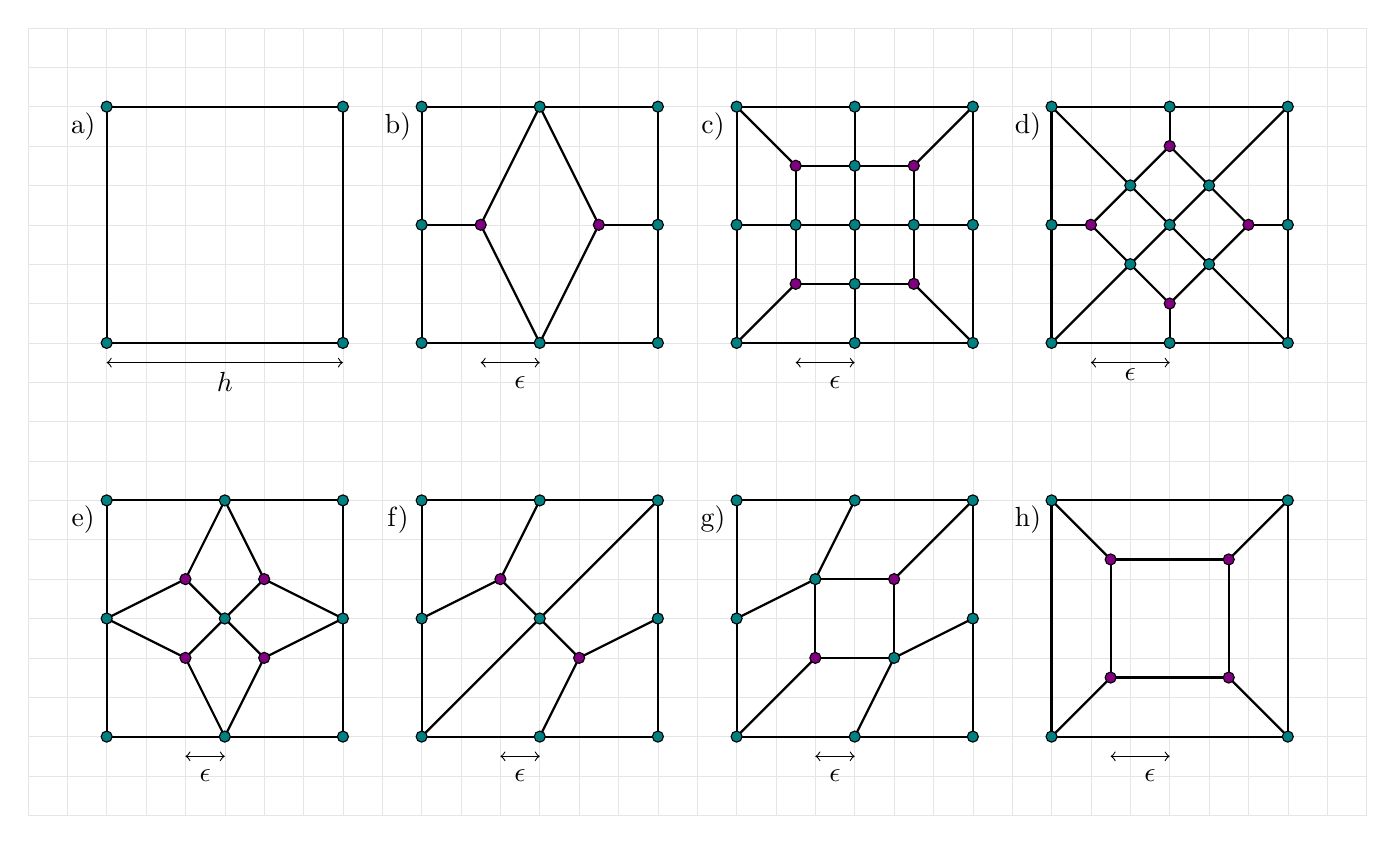
\begin{tikzpicture}
%\draw[fill=gray!23,gray!23](0,0) rectangle (5,5);
\draw[step=0.5cm,gray!20,very thin] (0,0) grid (17,10); %background grid

%%%%%%%%%%%%%%%%%%%%%%%%%%%%%%%%%%%%%%%%%%%%%%%%%%%%%%%%%%
\node[] at (0.7,3.75) {e)};
\draw[thick] (1,1) -- (4,1) -- (4,4) -- (1,4) -- cycle;  

\draw[thick] (1,2.5)--(2,3)--(2.5,4)--(3,3)--(4,2.5)--(3,2)--(2.5,1)--(2,2)--cycle;
\draw[thick] (2,2)--(3,3);
\draw[thick] (2,3)--(3,2);

\draw[black,fill=teal] (1,1)   circle (2pt);
\draw[black,fill=teal] (1,4)   circle (2pt);
\draw[black,fill=teal] (4,1)   circle (2pt);
\draw[black,fill=teal] (4,4)   circle (2pt);
\draw[black,fill=teal] (2.5,2.5)   circle (2pt);

\draw[black,fill=teal] (1,2.5)   circle (2pt);
\draw[black,fill=teal] (4,2.5)   circle (2pt);
\draw[black,fill=teal] (2.5,1)   circle (2pt);
\draw[black,fill=teal] (2.5,4)   circle (2pt);

\draw[black,fill=violet] (2,2)   circle (2pt);
\draw[black,fill=violet] (3,2)   circle (2pt);
\draw[black,fill=violet] (2,3)   circle (2pt);
\draw[black,fill=violet] (3,3)   circle (2pt);

\draw[<->] (2,0.75)--(2.5,0.75); \node[] at (2.25,0.5) {$\epsilon$};

%%%%%%%%%%%%%%%%%%%%%%%%%%%%%%%%%%%%%%%%%%%%%%%%%%%%%%%%%%%%%
\node[] at (4.7,3.75) {f)};
\draw[thick] (5,1) -- (8,1) -- (8,4) -- (5,4) -- cycle;  


\draw[thick] (6.5,1)--(7,2)--(8,2.5) ; 
\draw[thick] (5,2.5)--(6,3)--(6.5,4) ; 
\draw[thick] (6,3)--(7,2);
\draw[thick] (5,1)--(8,4);

\draw[black,fill=teal] (5,1)   circle (2pt);
\draw[black,fill=teal] (5,4)   circle (2pt);
\draw[black,fill=teal] (8,1)   circle (2pt);
\draw[black,fill=teal] (8,4)   circle (2pt);
\draw[black,fill=teal] (6.5,2.5)  circle (2pt);
\draw[black,fill=teal] (5,2.5)   circle (2pt);
\draw[black,fill=teal] (8,2.5)   circle (2pt);
\draw[black,fill=teal] (6.5,1)   circle (2pt);
\draw[black,fill=teal] (6.5,4)   circle (2pt);

\draw[black,fill=violet] (6,3)   circle (2pt);
\draw[black,fill=violet] (7,2)   circle (2pt);


\draw[<->] (6,0.75)--(6.5,0.75); \node[] at (6.25,0.5) {$\epsilon$};

%%%%%%%%%%%%%%%%%%%%%%%%%%%%%%%%%%%%%%%%%%%%%%%%%%%%%%%%%%%%%
\node[] at (8.7,3.75) {g)};
\draw[thick] (9,1) -- (12,1) -- (12,4) -- (9,4) -- cycle;  
\draw[thick] (10,2)--(11,2)--(11,3)--(10,3)--cycle; 
\draw[thick] (9,1)--(10,2);
\draw[thick] (11,3)--(12,4);
\draw[thick] (10.5,1)--(11,2)--(12,2.5);
\draw[thick] (9,2.5)--(10,3)--(10.5,4);

\draw[black,fill=teal] (9,1)   circle (2pt);
\draw[black,fill=teal] (10.5,1)   circle (2pt);
\draw[black,fill=teal] (12,1)   circle (2pt);
\draw[black,fill=teal] (9,2.5)   circle (2pt);
\draw[black,fill=teal] (12,2.5)   circle (2pt);
\draw[black,fill=teal] (9,4)   circle (2pt);
\draw[black,fill=teal] (10.5,4)   circle (2pt);
\draw[black,fill=teal] (12,4)   circle (2pt);
\draw[black,fill=teal] (10,3)   circle (2pt);
\draw[black,fill=teal] (11,2)   circle (2pt);

\draw[black,fill=violet] (10,2)   circle (2pt);
\draw[black,fill=violet] (11,3)   circle (2pt);


\draw[<->] (10,0.75)--(10.5,0.75); \node[] at (10.25,0.5) {$\epsilon$};



%%%%%%%%%%%%%%%%%%%%%%%%%%%%%%%%%%%%%%%%%%%%%%%%%%%%%%%%%%%
\node[] at (12.7,3.75) {h)};
\draw[thick] (13,1) -- (16,1) -- (16,4) -- (13,4) -- cycle;  


\draw[thick] (13.75,1.75)--(15.25,1.75)--(15.25,3.25)--(13.75,3.25)--cycle; 
\draw[thick] (13,1)--(13.75,1.75); 
\draw[thick] (16,1)--(15.25,1.75); 
\draw[thick] (13,4)--(13.75,3.25); 
\draw[thick] (16,4)--(15.25,3.25); 

\draw[black,fill=teal] (13,1)   circle (2pt);
\draw[black,fill=teal] (16,1)   circle (2pt);
\draw[black,fill=teal] (13,4)   circle (2pt);
\draw[black,fill=teal] (16,4)   circle (2pt);

\draw[black,fill=violet] (13.75,1.75)   circle (2pt);
\draw[black,fill=violet] (13.75,3.25)   circle (2pt);
\draw[black,fill=violet] (15.25,1.75)   circle (2pt);
\draw[black,fill=violet] (15.25,3.25)   circle (2pt);

\draw[<->] (13.75,0.75)--(14.5,0.75); \node[] at (14.25,0.5) {$\epsilon$};

%%%%%%%%%%%%%%%%%%%%%%%%%%%%%%%%%%%%%%%%%%%%%%%%%%%%%%%%%%%
\node[] at (0.7,8.75) {a)};
\draw[thick] (1,6) -- (4,6) -- (4,9) -- (1,9) -- cycle;  
\draw[black,fill=teal] (1,6)   circle (2pt);
\draw[black,fill=teal] (4,6)   circle (2pt);
\draw[black,fill=teal] (1,9)   circle (2pt);
\draw[black,fill=teal] (4,9)   circle (2pt);

\draw[<->] (1,5.75)--(4,5.75);
\node[] at (2.5,5.5) {$h$};

%%%%%%%%%%%%%%%%%%%%%%%%%%%%%%%%%%%%%%%%%%%%%%%%%%%%%%%%%%%
\node[] at (4.7,8.75) {b)};
\draw[thick] (5,6) -- (8,6) -- (8,9) -- (5,9) -- cycle;  
\draw[thick] (6.5,6)--(7.25,7.5)--(6.5,9)--(5.75,7.5) -- cycle;  
\draw[thick] (5,7.5) -- (5.75,7.5);  
\draw[thick] (7.25,7.5) -- (8,7.5);  
\draw[black,fill=teal] (5,6) circle (2pt);
\draw[black,fill=teal] (6.5,6) circle (2pt);
\draw[black,fill=teal] (8,6) circle (2pt);
\draw[black,fill=teal] (5,7.5) circle (2pt);
\draw[black,fill=violet] (5.75,7.5) circle (2pt);
\draw[black,fill=violet] (7.25,7.5) circle (2pt);
\draw[black,fill=teal] (8,7.5) circle (2pt);
\draw[black,fill=teal] (5,9) circle (2pt);
\draw[black,fill=teal] (6.5,9) circle (2pt);
\draw[black,fill=teal] (8,9) circle (2pt);

\draw[<->] (5.75,5.75)--(6.5,5.75); \node[] at (6.25,5.5) {$\epsilon$};


%%%%%%%%%%%%%%%%%%%%%%%%%%%%%%%%%%%%%%%%%%%%%%%%%%%%%%%%%%%%%
\node[] at (8.7,8.75) {c)};
\draw[thick] (9,6) -- (12,6) -- (12,9) -- (9,9) -- cycle;  
\draw[thick] (9.75,6.75)--(11.25,6.75)--(11.25,8.25)--(9.75,8.25) -- cycle;  

\draw[thick] (9,6) -- (9.75,6.75);  
\draw[thick] (11.25,8.25) -- (12,9);  
\draw[thick] (9,9) -- (9.75,8.25);  
\draw[thick] (11.25,6.75) -- (12,6);  
\draw[thick] (9,7.5) -- (12,7.5);  
\draw[thick] (10.5,6) -- (10.5,9);  

\draw[black,fill=teal] (9,6)  circle (2pt);
\draw[black,fill=teal] (10.5,6)  circle (2pt);
\draw[black,fill=teal] (12,6)   circle (2pt);
\draw[black,fill=teal] (9,7.5)  circle (2pt);
\draw[black,fill=teal] (10.5,7.5)  circle (2pt);
\draw[black,fill=teal] (12,7.5)   circle (2pt);
\draw[black,fill=teal] (9,9)  circle (2pt);
\draw[black,fill=teal] (10.5,9)  circle (2pt);
\draw[black,fill=teal] (12,9)   circle (2pt);

\draw[black,fill=teal] (10.5,8.25)   circle (2pt);
\draw[black,fill=teal] (10.5,6.75)   circle (2pt);
\draw[black,fill=teal] (9.75,7.5)   circle (2pt);
\draw[black,fill=teal] (11.25,7.5)   circle (2pt);

\draw[black,fill=violet] (9.75,6.75)  circle (2pt);
\draw[black,fill=violet] (11.25,6.75)  circle (2pt);
\draw[black,fill=violet] (9.75,8.25)  circle (2pt);
\draw[black,fill=violet] (11.25,8.25)  circle (2pt);


\draw[<->] (9.75,5.75)--(10.5,5.75); \node[] at (10.25,5.5) {$\epsilon$};


%%%%%%%%%%%%%%%%%%%%%%%%%%%%%%%%%%%%%%%%%%%%%%%%%%%%%%%%%%%
\node[] at (12.7,8.75) {d)};
\draw[thick] (13,6) -- (16,6) -- (16,9) -- (13,9) -- cycle;  

\draw[thick] (13,6) -- (16,9) ;
\draw[thick] (13,9) -- (16,6) ;

\draw[thick] (13.5,7.5)--(14.5,6.5)--(15.5,7.5)--(14.5,8.5) -- cycle;
\draw[thick] (13,7.5) -- (13.5,7.5) ;
\draw[thick] (15.5,7.5) -- (16,7.5) ;
\draw[thick] (14.5,6) -- (14.5,6.5) ;
\draw[thick] (14.5,8.5) -- (14.5,9) ;

\draw[black,fill=teal] (13,6)   circle (2pt);
\draw[black,fill=teal] (14.5,6)   circle (2pt);
\draw[black,fill=teal] (16,6)   circle (2pt);
\draw[black,fill=teal] (13,7.5)   circle (2pt);
\draw[black,fill=teal] (14.5,7.5)   circle (2pt);
\draw[black,fill=teal] (16,7.5)   circle (2pt);
\draw[black,fill=teal] (13,9)   circle (2pt);
\draw[black,fill=teal] (14.5,9)   circle (2pt);
\draw[black,fill=teal] (16,9)   circle (2pt);

\draw[black,fill=teal] (14,7)   circle (2pt);
\draw[black,fill=teal] (15,7)   circle (2pt);
\draw[black,fill=teal] (14,8)   circle (2pt);
\draw[black,fill=teal] (15,8)   circle (2pt);

\draw[black,fill=violet] (14.5,6.5)   circle (2pt);
\draw[black,fill=violet] (14.5,8.5)   circle (2pt);
\draw[black,fill=violet] (13.5,7.5)   circle (2pt);
\draw[black,fill=violet] (15.5,7.5)   circle (2pt);

\draw[<->] (13.5,5.75)--(14.5,5.75); \node[] at (14,5.6) {$\epsilon$};

\end{tikzpicture}

\caption{
a) velocity nodes for a $Q_1\times P_0$ R macro-element;
b) Stenberg (S) macro-element \cite{sten84}; 
c) Le Tallec (LT) macro-element \cite{leta81,leru86}; 
d,e,f) Qin \& Zhiang (QZ1, QZ2, and QZ3) macro-elements \cite{qizh07}; 
g,h) newly proposed macro-elements T1 and T2 (this study).
Velocity nodes are represented by filled-in circles: 
the purple ones indicate internal nodes which belong to 3 elements.
\label{fig:mes}}
\end{figure}

Concerning the new macro-elements T1 and T2 proposed by the author, they have not been proven stable. 
They are arrived at by studying the other existing ones and making sure that they contain at 
least one node that belongs to three elements so as to hamper checkerboard modes.

%checkerboard: US
%chequerboard: UK

Looking  at Fig.~\ref{fig:mes}, we can also make the observation that some macro-elements 
have a two-fold symmetry (along the axis or the diagonals) while others have a four-fold one 
(axis and diagonals). May be more important is the fact that S, QZ3 and T1 are `anisotropic', i.e., in 
the case of QZ3 for example, there are edges joining two opposite corners of the macro-element
but none joining the other two opposite corners.
In Table~\ref{tab1} I summarize the various properties which characterizes each macro-element.

\begin{table}
\centering
\begin{tabular}{cp{2cm}p{2cm}p{2.5cm}p{2cm}p{2cm}p{2cm}}
\hline
{name} & {axes symmetry}  & {diagonals symmetry} & {\# nodes inside} 
& {\# elements per m-e} & {mid edge points} & equal area \\
\hline
\hline
R,Rp,Rrp   &  Yes &  Yes & 1  & 4 & No  & Yes\\
S   &  Yes &   No & 2  & 5 & Yes & Yes\\
LT  &  Yes &  Yes & 9 & 12 & Yes & Yes\\
QZ1 &  Yes &  Yes & 9 & 12 & Yes & Yes\\
QZ2 &  Yes &  Yes & 5 & 8  & Yes & No\\
QZ3 &  No  &  Yes & 3 & 6  & Yes & Yes\\
T1  &  No  &  Yes & 4 & 7  & Yes & No\\
T2  &  Yes &  Yes & 4 & 5  & No  & Yes\\
\hline
\end{tabular}
\caption{Characteristics of all 8 macro-elements as shown in Fig.~\ref{fig:mes}.\label{tab1}}%
\end{table}

The stability of a velocity-pressure pair or a macro-element is often difficult to prove 
and various techniques have been proposed \cite{bobf13}. 
All 5 previously published macro-elements (R,LT,QZ1,QZ2,QZ3) were shown to be LBB-stable and all showcase at least 
an internal node shared by an odd number of elements which makes a checkerboard pattern impossible. 
However, things are not that simple since macro-element T2 showcases 
4 such points and as we will see it is not stable and checkerboard patterns still occur 
albeit at the macro-element scale\footnote{See appendix B} 
so that their presence therefore seems to be necessary but not sufficient to determine whether 
a macro-element is LBB-stable or not. 

Finally Qi et al \cite{qizh07} state "[...] from the points of implementation and the approximation property, we 
would list five types of macro-elements from the best to worst as S, LT, QZ1, QZ2, QZ3." 
The authors unfortunately do not provide any numerical comparison between these 5 and their 
ranking is therefore not borne by hard evidence. Furthermore, we will find that our ranking disagrees with theirs. 
%Understand what their ranking is based on. My pragmatic approach - numerical testing!

\paragraph{A remark about the QZ1 and QZ3 macro-elements:}
Let us consider the triangular macro-element as shown in Fig.~\ref{fig:triangle}.
As mentioned in \cite{rovira1992}, 
the velocity and pressure spaces in this case are isomorphic to those
of the $P_2^+ \times P_{-1}$ element \cite{thba25}. Since this velocity-pressure pair 
element satisfies the LBB condition, the macroelement depicted in this figure
composed of $Q_1 \times P_0$ elements is also div-stable.
One could in principle then generate a mesh of simplices and then subdivide those into 
three quadrilaterals to arrive at a mesh composed of stable macro-elements.
This avenue will not be pursued here. Finally I show in Appendix A that QZ1 and QZ3 are related.

\begin{figure}
\centering
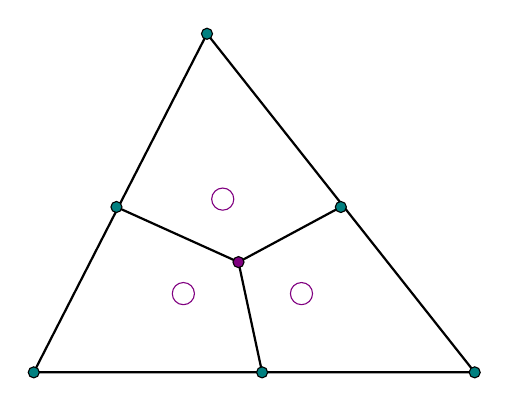
\begin{tikzpicture}
\draw[thick] (0,0) -- (5.6,0) -- (2.2,4.3)-- cycle;  
\draw[thick] (1.05,2.1) -- (2.6,1.4) -- (3.9,2.1);  
\draw[thick] (2.6,1.4) -- (2.9,0);  
\draw[black,fill=teal] (0,0) circle (2pt);
\draw[black,fill=teal] (5.6,0) circle (2pt);
\draw[black,fill=teal] (2.2,4.3) circle (2pt);
\draw[black,fill=teal] (1.05,2.1) circle (2pt);
\draw[black,fill=violet] (2.6,1.4) circle (2pt);
\draw[black,fill=teal] (3.9,2.1) circle (2pt);
\draw[black,fill=teal] (2.9,0) circle (2pt);
\draw[violet] (1.9,1) circle (4pt);
\draw[violet] (3.4,1) circle (4pt);
\draw[violet] (2.4,2.2) circle (4pt);
\end{tikzpicture}
\caption{A triangular macro-element made of 3 $Q_1\times P_0$ elements.
Green discs correspond to velocity nodes while open circles 
correspond to pressure dofs.}\label{fig:triangle}
\end{figure}

\vspace{.4cm}


In the end, despite the existing literature, many questions remain with regards to these macro-elements:
\begin{itemize}
\item Based on a handful of analytical benchmarks is it possible to establish a ranking, 
or at the very least can we pinpoint the objectively worse one(s)?

%\item Is there an optimal position for the additional internal nodes? (i.e. can we 
%determine an optimal value of the 
%$\epsilon$ parameter for each macro-element?)

\item Can these macro-elements be safely used for geodynamical 
buoyancy-driven flows in the presence of a strong hydrostatic pressure gradient?

\item How do the (best) macro-elements compare with the simple approach of 
distorted/randomized meshes?

\item Which of the common pressure filtering/smoothing methods found in the literature is the most accurate?
\end{itemize}











%%%%%%%%%%%%%%%%%%%%%%%%%%%%%%%%%%%%%%%%%%%%%%%%%%%%%%%%%%%%%%%%%%%%%%%%%5
\section{Implementation}


For the purpose of this paper, we are concerned with the numerical solution of 
the incompressible and isothermal Stokes equations:
\begin{eqnarray}
-\nabla \cdot \left[ 2\eta \varepsilon({\bm u}) \right] + \nabla p &=& \rho \bm g \qquad  \textrm{in $\Omega$},
\label{eq:conv_momentum}  \\  
-\nabla \cdot {\bm u} &=& 0    \qquad    \textrm{in $\Omega$},   \label{eq:conv_mass} 
\end{eqnarray}
where $\eta$ is the viscosity, $\rho$ the density, ${\bm g}$ the gravity vector, $\varepsilon(\cdot)$
denotes the symmetric gradient operator defined by $\varepsilon({\bm u})
=\frac 12 (\nabla {\bm u} + \nabla {\bm u}^{T})$, 
and $\Omega\subset{\mathbb R}^2$ is the domain
of interest. Both the viscosity $\eta$
and the density $\rho$ will, in general, be spatially variable.

The Stokes equations are discretised using the Finite Element Method.
and the unknowns are the velocity vector ${\bm u}$ and the pressure $p$ so that 
one speaks of a Mixed Finite Element method. 
A straightforward application of the Galerkin method yields the finite-dimensional 
variational problem: 
\textit{Find ${\bm u}_h\in {\cal Q}_1,p_h\in {\cal Q}_0$
so that
\begin{eqnarray}
\label{eq:discrete-formulation}
\left(\varepsilon(\bm v_h), 2\eta \varepsilon(\bm u_h)\right)  
- ( \nabla \cdot \bm v_h, p_h) &=&   ({\bm v}_h,\rho \bm g),\\
-(q_h,\nabla \cdot \bm u_h) &=& 0,
\end{eqnarray}
for all test functions ${\bm v}_h\in {\cal Q}_1, q_h\in {\cal Q}_0$.}
This procedure is rather standard and well documented in many 
textbooks \cite{grsa,dohu03,bobf13} and the reader is referred to these sources 
for more detail.

All (macro-)elements have been implemented in a dedicated Python code (see Supplementary material). 
An isoparametric mapping is used and the fully assembled Stokes matrix is passed to the 
default SciPy Python solver. 
Better solving strategies have of course 
been designed to solve the resulting saddle point \cite{begl05} but are not 
implemented since optimal performance is not of interest here.
The pressure nullspace due to the Dirichlet boundary conditions on all sides is removed 
after the linear system is solved, by imposing $\int_\Omega p dV= 0$.
In the case of non-isoviscous experiments the viscosity is computed at each 
quadrature point. The gradient and divergence blocks in the FE Stokes matrix are
scaled as explained for example in step 32 of the deal.II library\footnote{\url{https://www.dealii.org/9.0.0/doxygen/deal.II/step_32.html}}.

The projection of the discontinuous pressure $p$ onto the velocity nodes is denoted by $q$. 
Techniques how to do so (and thereby filter out the checkerboard modes) have been presented 
for example in \cite{legs79,sagl81a,chpc95,thfb08}.
For simplicity, and since all elements have equal or very similar areas 
I have adopted the following simple procedure: each 
elemental pressure is multiplied by a given weight and is added to the nodes making 
this element and later averaged: the pressure at a node is then given by
\[
q = \frac{1}{n} \sum_{e=1}^{n} \xi_e p_e
\]
where $n$ is the number of elements to which the node belongs.
We find multiple options in the literature for the weight $\xi_e$.
We shall not embark on a full detailed study of all the possibilities 
and instead will consider three nodal pressure calculations:
a) $q_1$ is obtained when $\xi_e=1$, i.e. a simple arithmetic average; 
b) $q_2$ is obtained when $\xi_e=A_e$ where $A_e$ is the area of element $e$
(scheme 3 of \cite{sagl81a}).
b) $q_3$ is obtained when $\xi_e=A_e^T$ where $A_e^T$ is the area of the triangle cutting
element $e$ along the diagonal for which the node belongs to two edges (scheme 2 of \cite{sagl81a}).
{\color{blue} W: figure needed?}

When an analytical solution exists error convergence rates are computed and 
we expect for smooth viscosity fields and/or boundary conditions that the convergence rates 
are optimal, i.e., that the errors satisfy the relationships
\begin{eqnarray}
\| {\bm u} - {\bm u}_h \|_{L_2} &=&  {\cal O}(h^{2}),     \\  
\| p - p_h \|_{L_2}   &=& {\cal O}(h^{1}),
  \label{eq:error-rates}
\end{eqnarray}
where $h$ is commonly defined as the cell size.
Looking at Fig.~\ref{fig:mes} we see that the elements inside the macro-elements 
have various sizes and shapes so 
the default version of each macro-element is the one for which all internal elements have the same area
(when possible -- see appendix C), and I then define the average element size
$h$ as the square root of the average elemental area.
{\color{blue} W: is this ok? should I take the longest of the diagonals of elements?}
I will also measure and report on the convergence rate index for the nodal pressure $q_1,q_2,q_3$.


%%%%%%%%%%%%%%%%%%%%%%%%%%%%%%%%%%%%%%%%%%%%%%%%%%%%%%%%%%%%%%%%%%
\section{The Donea \& Huerta manufactured solution as test case}

To test the implementation I first consider the manufactured solution 
proposed in Chapter 6 of \cite{dohu03} and also used in \cite{thba22,thba25}.
It will used to study all 7 macro-elements (S, LT, QZ1, QZ2, QZ3, T1, T2)
and all 4 regular mesh configuations (R, Rp, Rrp, FR) and draw conclusions 
that will allow us to eliminate a few from the rest of this article.
 
The domain is a unit square. The viscosity is constant and set to $\eta=1$.
The velocity and pressure fields are given by
\begin{eqnarray}
u_x(x,y) &=& x^2(1- x)^2 (2y - 6y^2 + 4y^3)  \\
u_y(x,y) &=& -y^2 (1 - y)^2 (2x - 6x^2 + 4x^3) \\
p(x,y) &=& x(1 -x)- 1/6. 
\end{eqnarray}
The buoyancy force is obtained by inserting these expressions in Eq.~(\ref{eq:conv_momentum}).
Boundary conditions are no-slip on all sides of the domain.
The velocity and pressure fields are shown in Fig.~\ref{fig:dh1}a,d.

\begin{figure}[t]
\centering
a)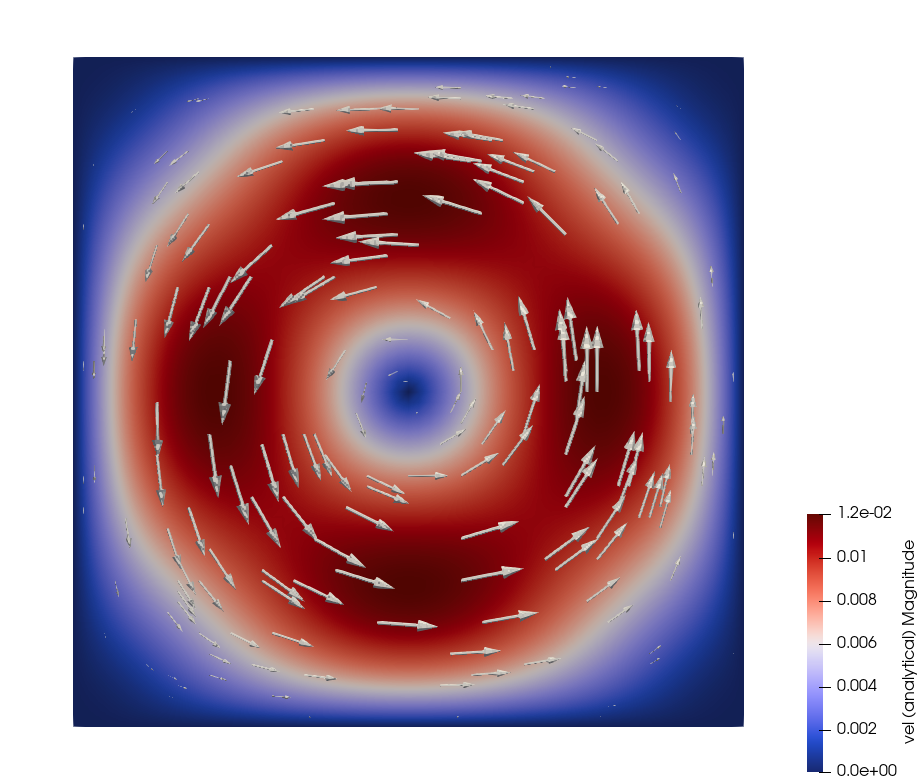
\includegraphics[width=5cm]{../images/fields/vel_dh}
b)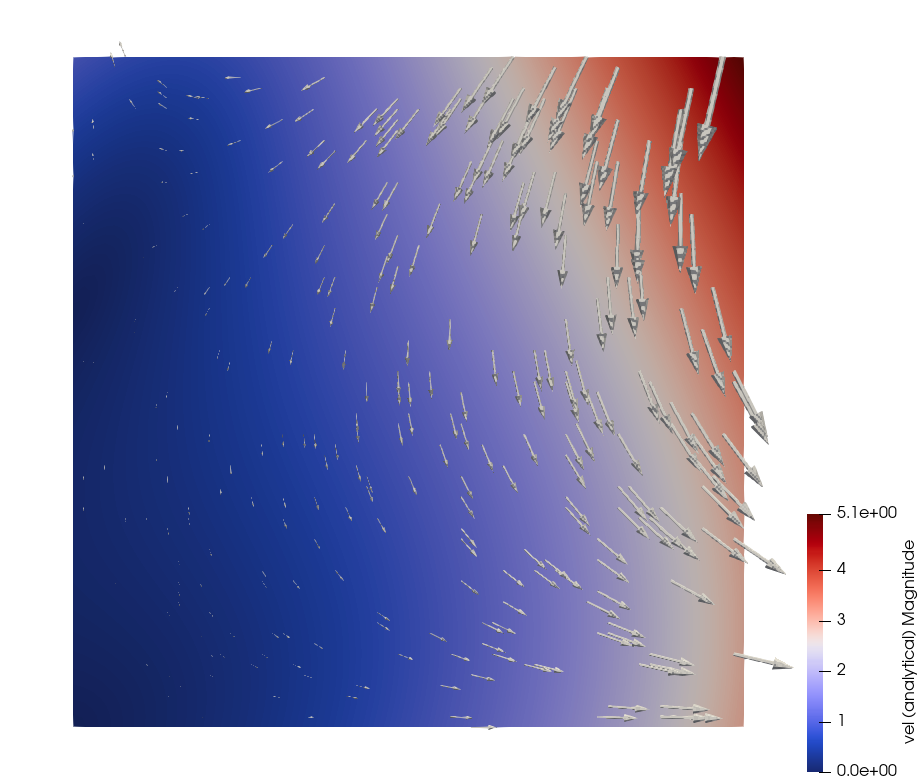
\includegraphics[width=5cm]{../images/fields/vel_dobo}
c)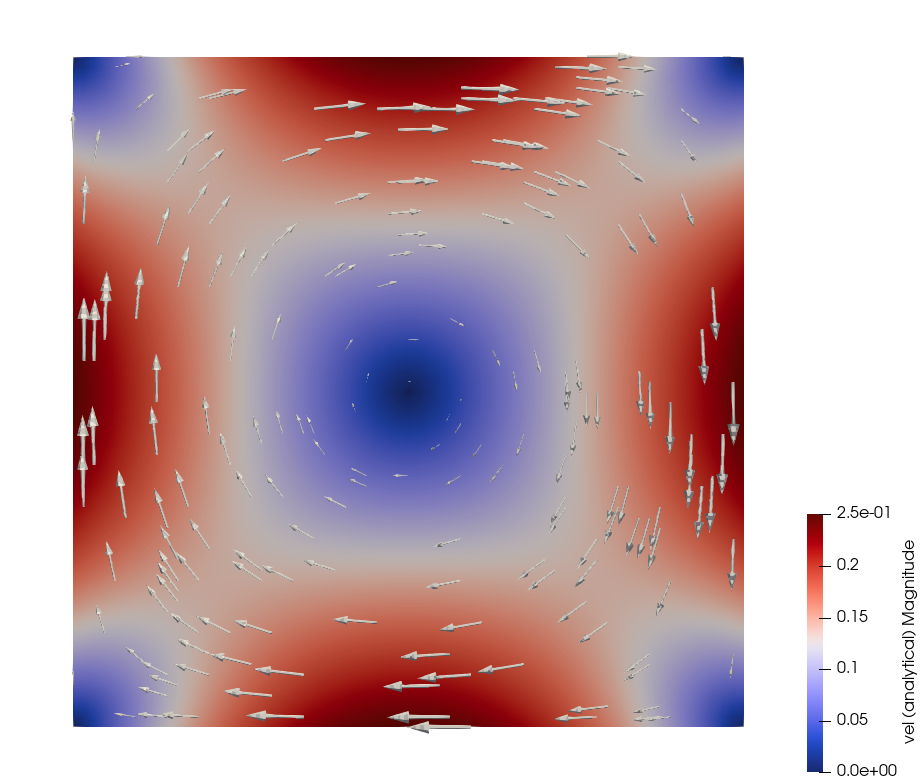
\includegraphics[width=5cm]{../images/fields/vel_cavity} \\
d)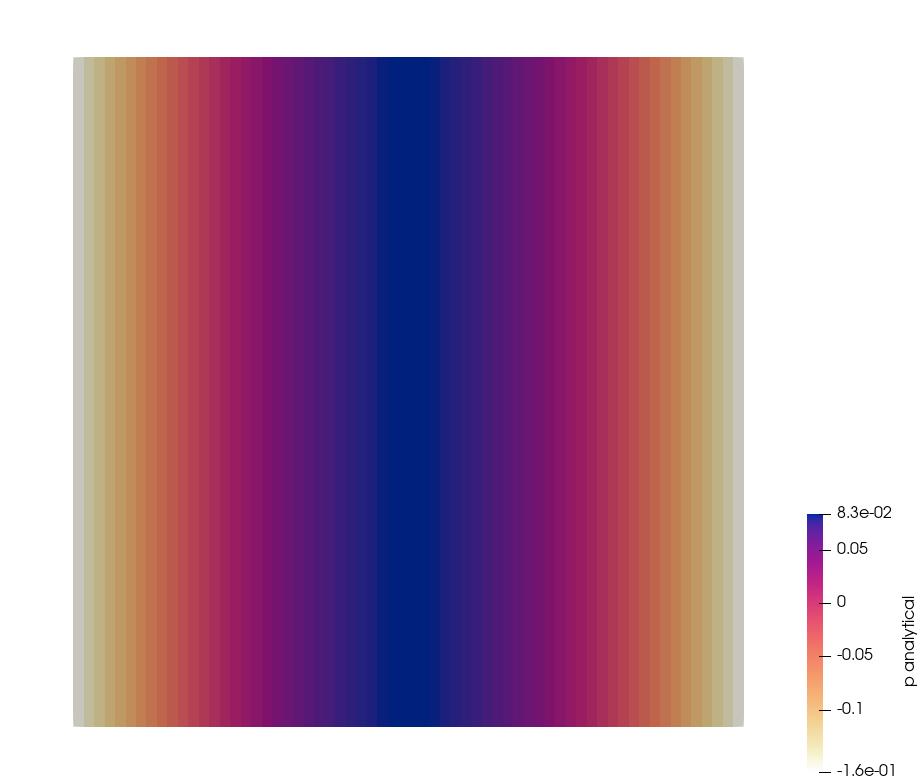
\includegraphics[width=5cm]{../images/fields/press_dh}
e)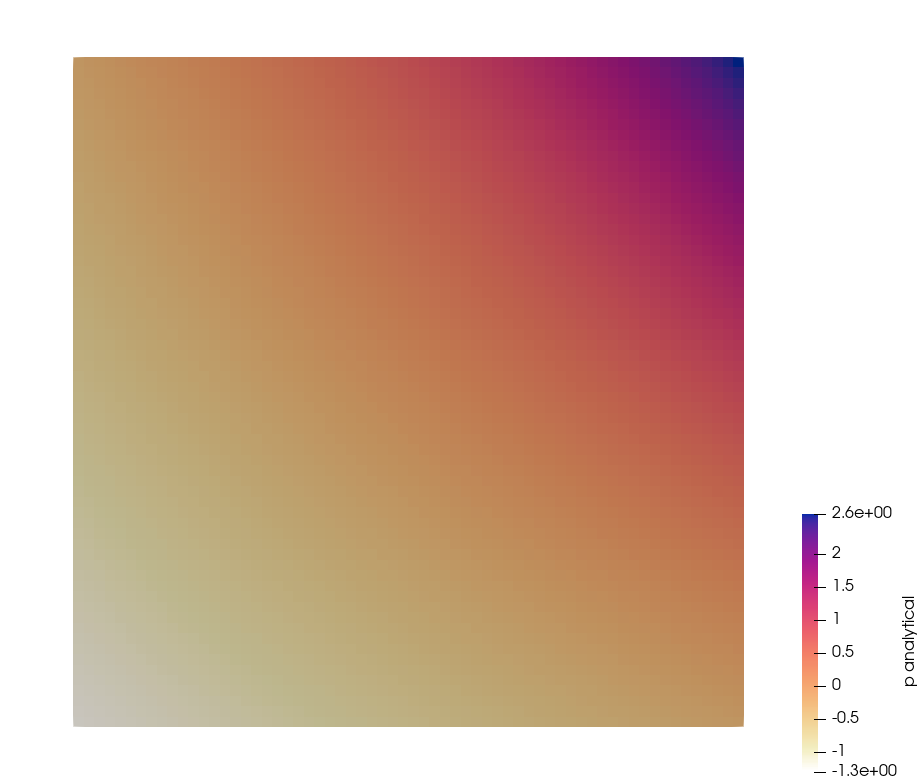
\includegraphics[width=5cm]{../images/fields/press_dobo}
f)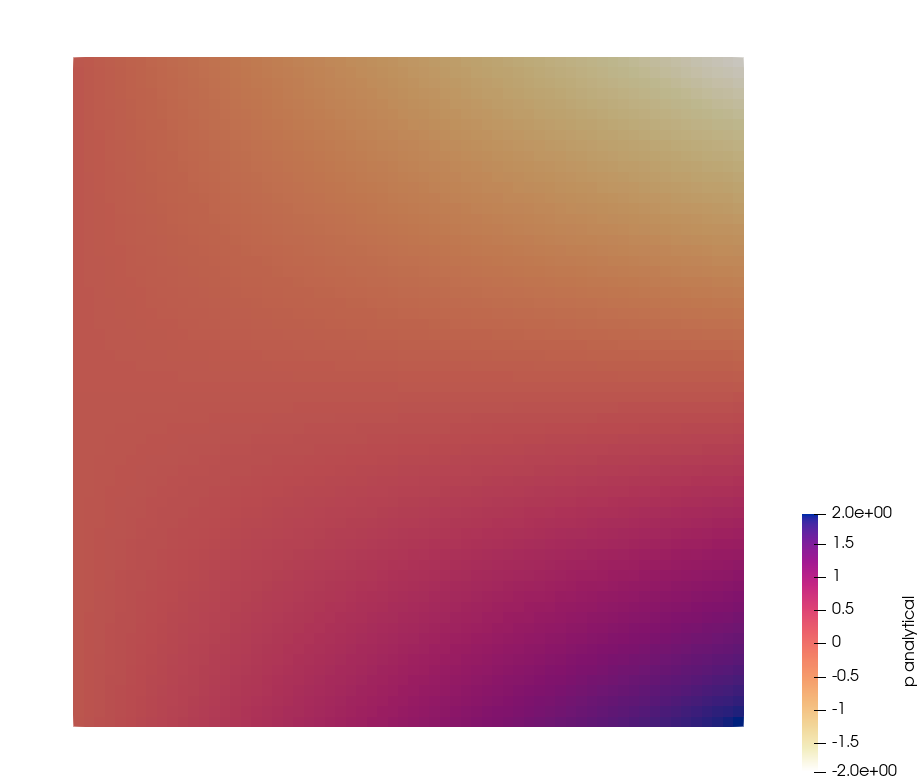
\includegraphics[width=5cm]{../images/fields/press_cavity}
\caption{Velocity field (top row) and pressure field (bottom 
row) for the three isoviscous manufactured solutions (a: Donea \& Huerta, 
b: Dohrmann \& Bochev, c: cavity) in this work. \label{fig:dh1}}
\end{figure}

\begin{figure}
\centering
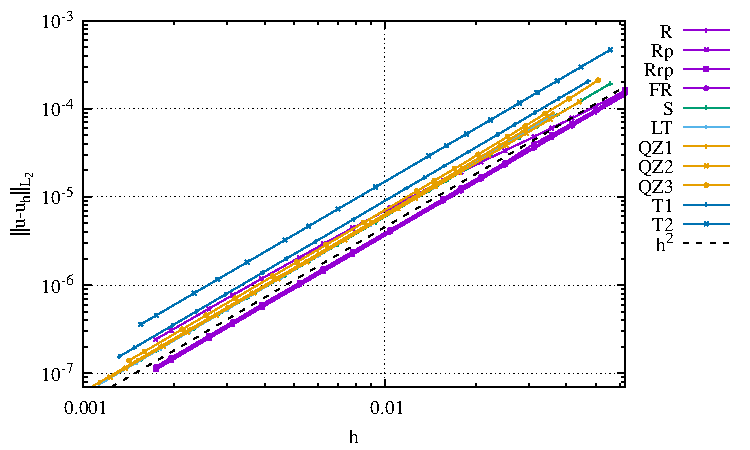
\includegraphics[width=8.9cm]{../results/errors_u_exp1}
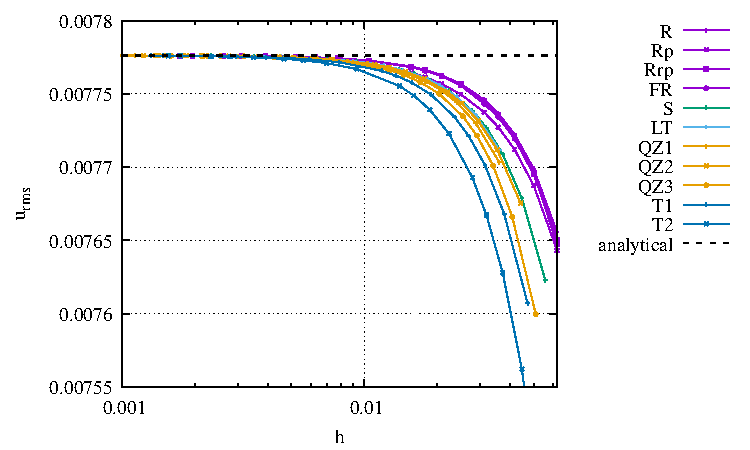
\includegraphics[width=8.9cm]{../results/vrms_exp1} \\
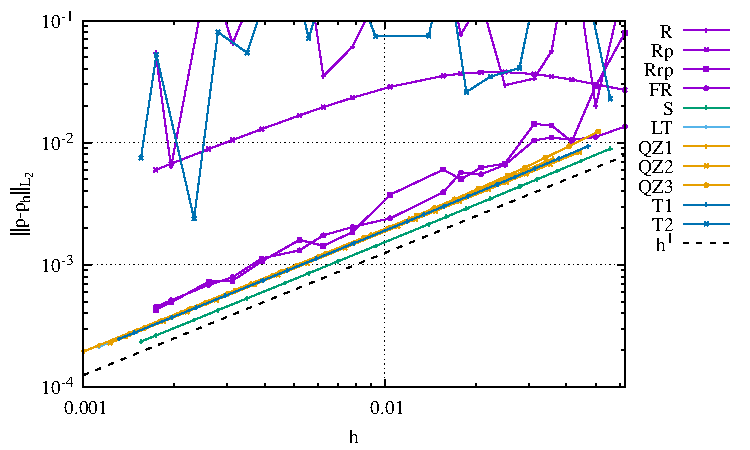
\includegraphics[width=8.9cm]{../results/errors_p_exp1}
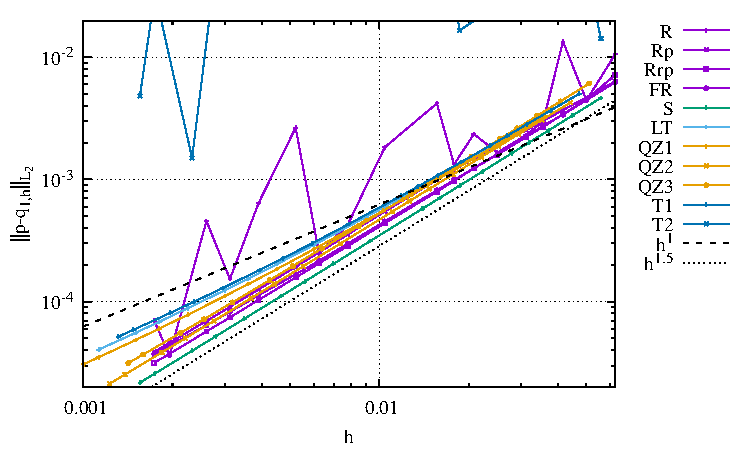
\includegraphics[width=8.9cm]{../results/errors_q1_exp1}\\
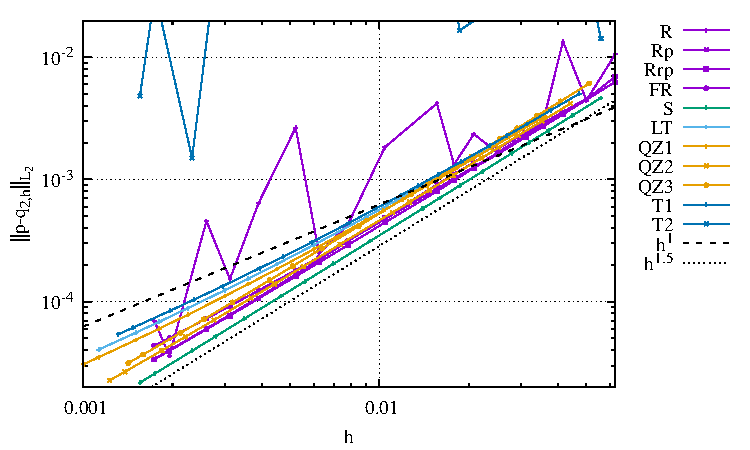
\includegraphics[width=8.9cm]{../results/errors_q2_exp1}
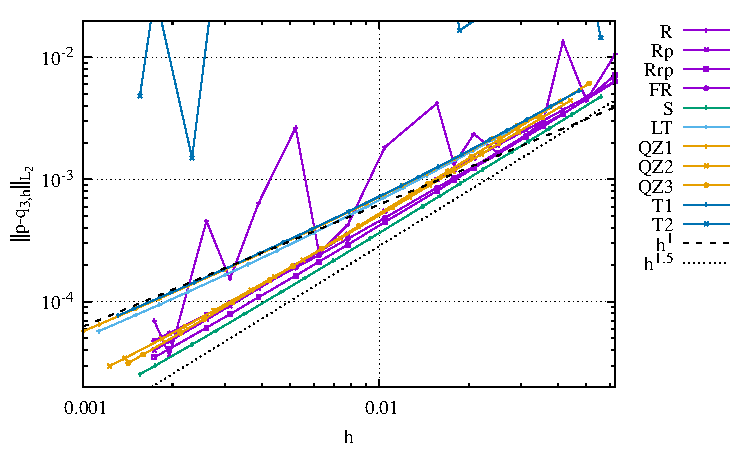
\includegraphics[width=8.9cm]{../results/errors_q3_exp1}
\caption{Donea and Huerta benchmark: velocity error, 
root mean square velocity, elemental pressure error and nodal pressure $q_1,q_2,q_3$ errors 
as a function of the the mesh size $h$.} 
\label{fig:resdh}
\end{figure}

In Fig.~\ref{fig:resdh} the velocity and pressure errors are shown as a function of the 
mesh size $h$ for all meshes.

\begin{itemize}

%comment on velocity
\item We recover the optimal (quadratic) convergence rate` for the velocity error for all meshes.
The R, Rrp and FR meshes are the most accurate, followed by the S, LT, QZ1, QZ2, QZ3 macro-elements
(all very close), while the T1 and T2 macro-elements are the least accurate ones. 
We note that the Rp mesh is substantially less accurate than the other R, Rrp and FR ones.

%comment on vrms
\item All meshes converge to the correct analytical root mean square velocity $u_{rms}$ and 
their accuracy follows the previously made observations on their respective velocity errors
(Fig.~\ref{fig:resdh}b).

%comment on elemental pressure p
\item As expected the 'R' macro-element yields a pressure field showcasing a checkerboard so that 
the corresponding pressure error does not decrease with increasing $h$ and behaves unpredictably
from one resolution to the other. Indeed, the amplitude of checkerboard modes is difficult to predict (it is a function 
of boundary conditions, mesh topology, even or odd numbers of elements per direction, flow features, ...) [REF?] 
\item The same observation can be made for macro-element T2. 
\item All other macro-elements pressure errors converge linearly and the S macro-element is
the most accurate of them all.
The Rp mesh converges linearly albeit with pressure errors an order of magnitude higher than 
the macro-elements.
\item Rrp and FR yield similar pressure errors which (on average) decrease linearly but the corresponding 
lines are broken, indicating that pressure modes are probably present. 
{\color{blue} W: Should I add the following figure?}

\begin{center}
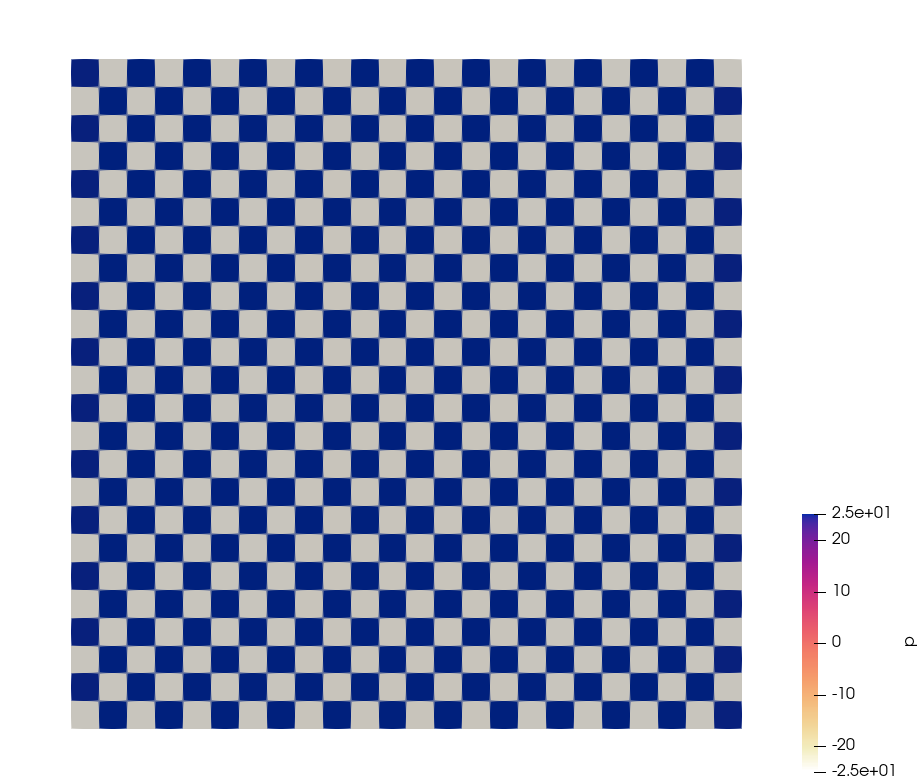
\includegraphics[width=5cm]{../results/exp01/p_topo0_24x24.png}
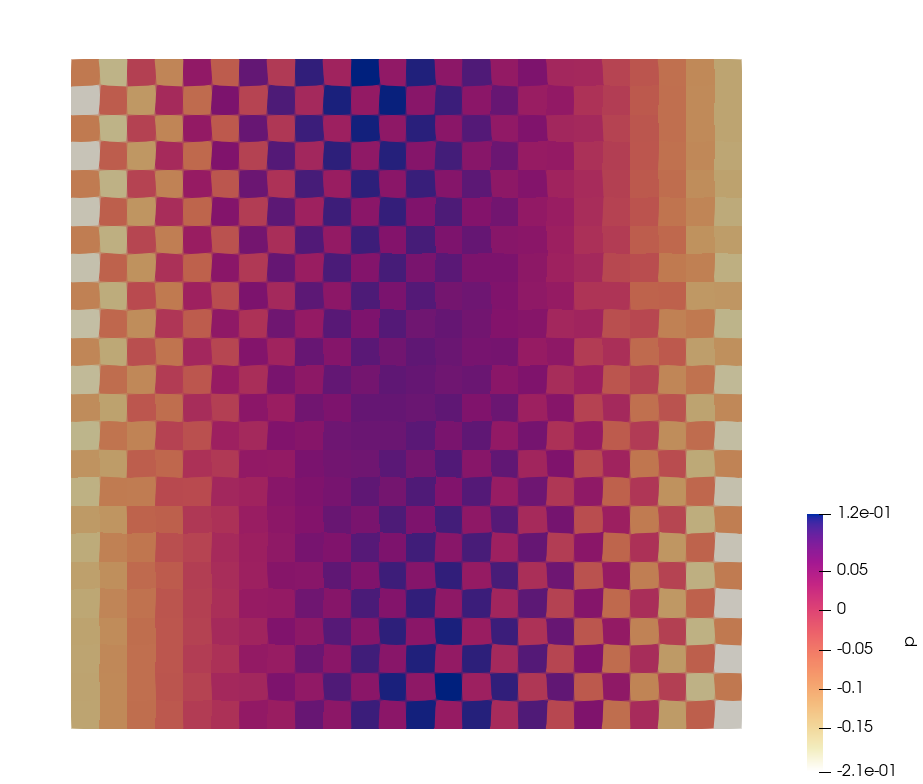
\includegraphics[width=5cm]{../results/exp01/p_topo8_24x24.png}
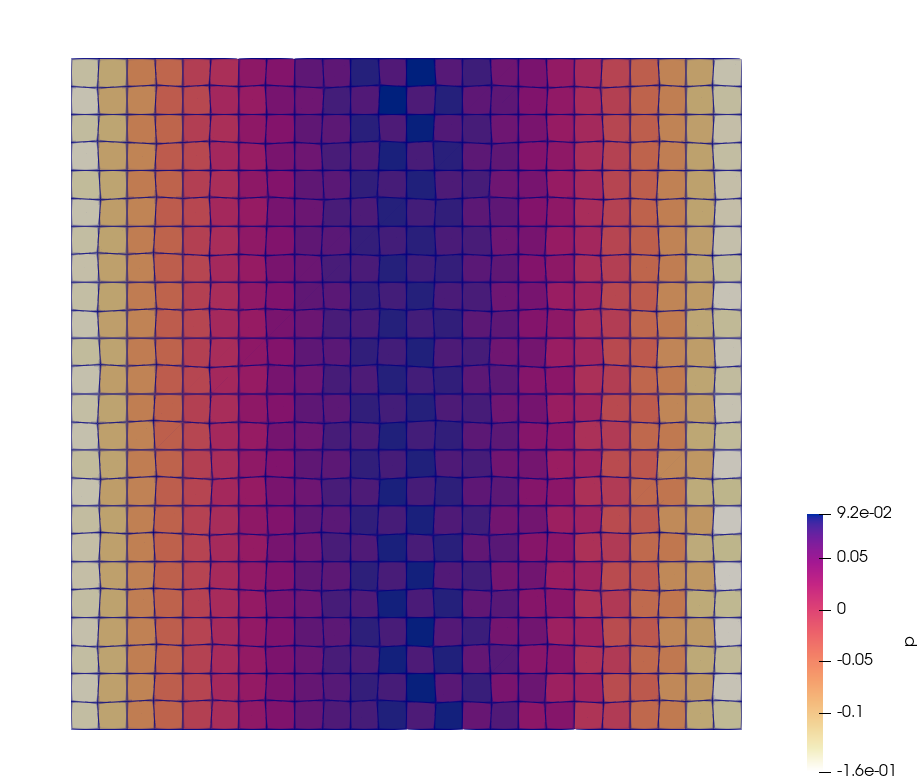
\includegraphics[width=5cm]{../results/exp01/p_topo9_24x24.png}\\
elemental pressure on a 24x24 mesh. From left to right: R, Rp, Rrp.
\end{center}



%comment on nodal pressure q
\item Looking at the $q1$, $q2$ and $q3$ errors, we see that 
$q_3$ errors are the highest of the three, with slightly lower convergence rates.
Comparing $q_1$ and $q_2$ error rates we find that $q_1$ errors are smaller and the 
rates higher.

\item Most meshes lead to nodal pressure error rates that converge ${\cal O}(h^{1.5})$, 
with the exception of LT, QZ1 and T1 which seem to converge linearly.
\item The Stenberg macro element S yields the most accurate elemental and nodal pressure
of all stable macro-elements. 

\end{itemize}



%As a conclusion, S is the clear best macro-element, followed by QZ2 and QZ3 macro-elements.

In the light of these observations we make the following choices pertaining to the 
numerical experiments that are subsequently carried out.
a) The $q_1$ approch is preferred and the other two $q_2$ and $q_3$ are discarded;
b) The newly-proposed macro-element T2 is not stable as the checkboard pattern was clearly observed
and translates into the broken line of Fig.~\ref{fig:resdh}c. This macro-element also yields the worst 
velocity error here and it is therefore abandoned. 
c) Rp is also abandoned: its velocity error is larger than Rrp for example, but 
more importantly its pressure error is more than 10x larger than the one of Rrp.
FR is also discarded: it yields virtually identical results as Rrp, but the $q_{1,2,3}$ errors for Rrp 
are slightly lower than FR. Also Rrp fits better the narrative of this paper  
which primarily focuses on macro-elements than FR.

Taking these facts into account we investigate 2 more similar manufactured solutions 
in the following section. 

%%%%%%%%%%%%%%%%%%%%%%%%%%%%%%%%%%%%%%%%%%%%%%%%%%%%%%%%%%%%%%%%%%
\section{Other isoviscous manufactured solutions}


%experiment=9
The second manufactured solution originates in Dohrmann \& Bochev \cite{dobo04} 
and the smooth exact solution is
\begin{eqnarray}
u_x(x,y) &=& x+x^2 - 2xy+x^3 - 3xy^2 + x^2y \\
u_y(x,y) &=& -y-2xy+y^2 -3x^2y + y^3 - xy^2 \\
p(x,y) &=& xy+x+y+x^3y^2 - 4/3
\end{eqnarray}
Here too the buoyancy terms can be obtained by inserting these expressions
in Eq.~(\ref{eq:conv_momentum}).
The analytical velocity is prescribed on all sides of the domain.
The velocity and pressure fields are shown in Fig.~\ref{fig:dh1}b,e.
Note that in this case the applied boundary conditions were slightly
altered so as to insure $\int_\Gamma {\bm u}\cdot{\bm n} dS =0$ [REF].
Discretization errors measurements are shown in Fig.~\ref{fig:resexp9}.

\begin{figure}
\centering
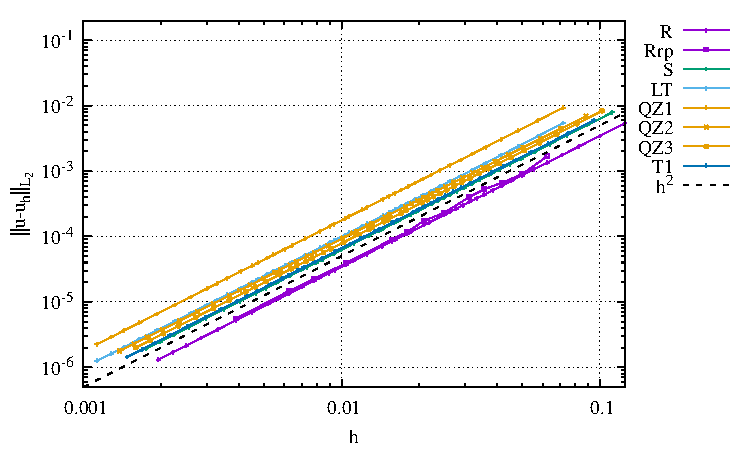
\includegraphics[width=8.9cm]{../results/errors_u_exp9}
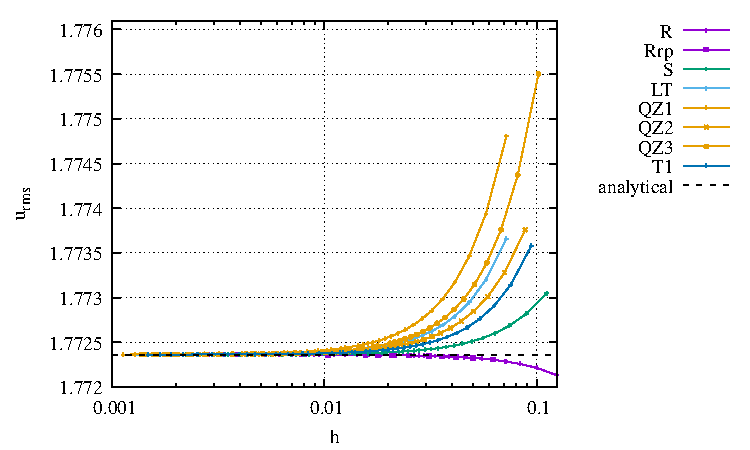
\includegraphics[width=8.9cm]{../results/vrms_exp9} \\
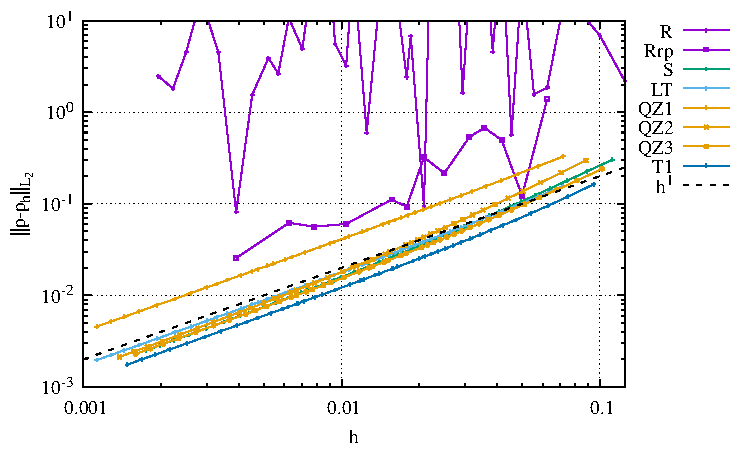
\includegraphics[width=8.9cm]{../results/errors_p_exp9}
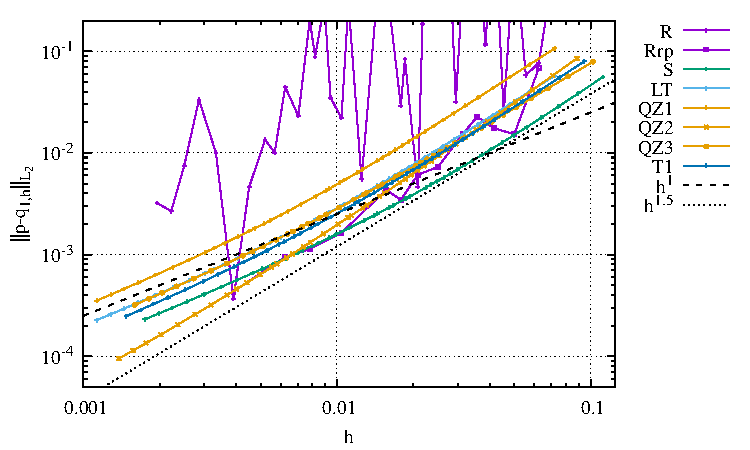
\includegraphics[width=8.9cm]{../results/errors_q1_exp9}
\caption{Dohrmann \& Bochev benchmark: velocity error, 
root mean square velocity, elemental pressure error and nodal pressure $q_1$ error
as a function of the mesh size $h$.} 
\label{fig:resexp9}
\end{figure}

From the results we conclude that
\begin{itemize}
\item velocity errors converges quadratically for all macro-elements.
The most accurate meshes are R and Rrp, the least accurate QZ1.
\item elemental pressure errors converge linearly for all macro-elements. R 
showcases the presence of spurious modes while Rrp seems again to converge linearly
albeit in a not so regular way. 
The most accurate is T1, the least accurate is QZ1.
\item the nodal pressure error converges as $h^{1.5}$ at low resolutions but ultimately 
the rate falls back to $h^1$ except for QZ2. 
\end{itemize}


%experiment=7
The third benchmark is a convection cell in a cavity and can be found in Elman et al \cite{elsw}.
The gravity is vertical with $\vec{g}=-\vec{e}_y$, and 
density is given by $\rho(x,y)=8x-2$. The velocity and pressure fields are given by
\begin{eqnarray}
u_x(x,y) &=&  (2y-1)x(1-x) \\
u_y(x,y) &=& - (2x-1)y(1-y) \\
p(x,y) &=& 2x(1 - 2y)
\end{eqnarray}
The analytical velocity is prescribed on the edges of the domain. 
The velocity and pressure fields are shown in Fig.~\ref{fig:dh1}c,f
and discretization errors are shown in Fig.~\ref{fig:resexp7}.

\begin{figure}
\centering
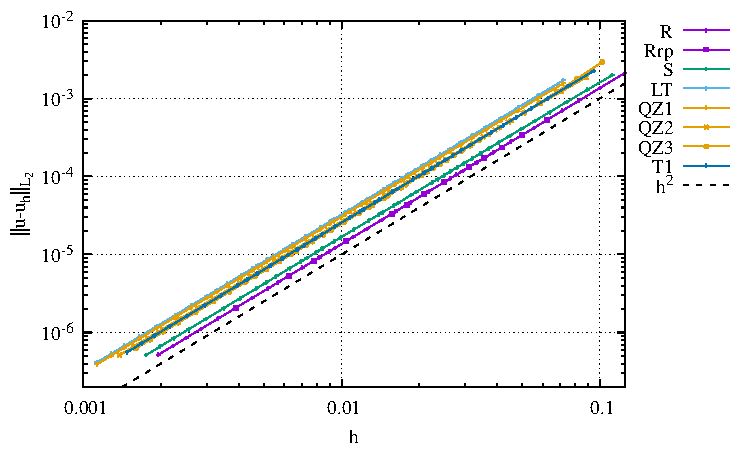
\includegraphics[width=8.9cm]{../results/errors_u_exp7}
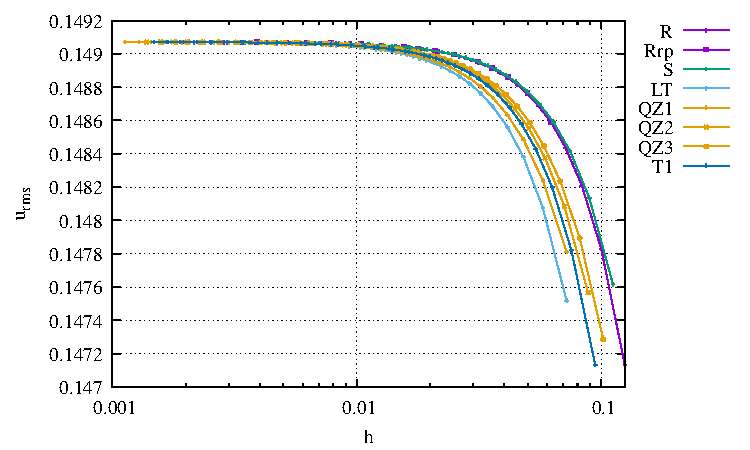
\includegraphics[width=8.9cm]{../results/vrms_exp7} \\
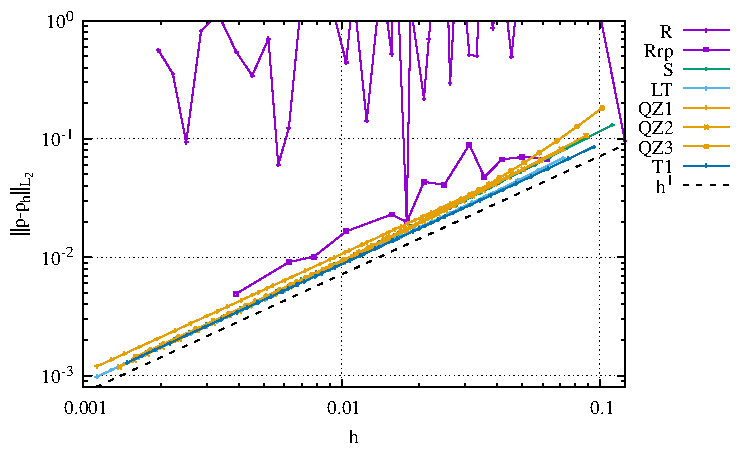
\includegraphics[width=8.9cm]{../results/errors_p_exp7}
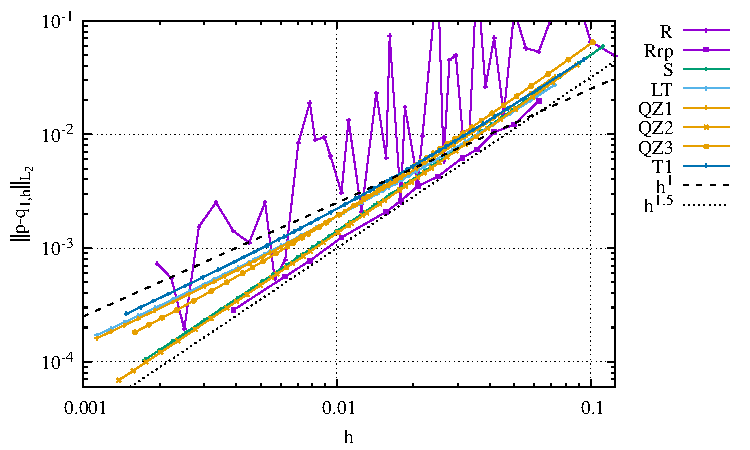
\includegraphics[width=8.9cm]{../results/errors_q1_exp7}
\caption{Elman et al benchmark: velocity error, 
root mean square velocity, elemental pressure error and nodal pressure $q_1$ error
as a function of the mesh size $h$.{\color{red} todo: add analytical value to urms}}
\label{fig:resexp7}
\end{figure}

We conclude that 
\begin{itemize}
\item Velocity error converges quadratically for all meshes. R, Rp and S are the most accurate.
\item elemental pressure errors converge linearly for all macro-elements, except R.
Rrp errors also decrease linearly but again in a broken line. 
QZ1 is the least accurate while all other macro-elements
yield nearly identical pressure errors.
\item This time nodal pressure errors for S and QZ2 and Rrp converge as $h^{1.5}$
while all others converge linearly.
\end{itemize}


{\color{red} write sentence to introduce/link with next section}


%%%%%%%%%%%%%%%%%%%%%%%%%%%%%%%%%%%%%%%%%%%%%%%%%%%%%%%%%%
\section{Non-isoviscous manufactured solutions}

The following two manufactured solutions (commonly called SolKz and SolCx in the 
geodynamics literature) are standard benchmarks in the computational geodynamics 
community \cite{mozg96,mamo08,krhb12,gemd13,demh19,thba22}.
The analytical solutions are derived in \cite{zhon96} and are available in open source codes
such as for example ASPECT\footnote{\url{https://github.com/geodynamics/aspect}} or 
Underworld2\footnote{\url{https://github.com/underworldcode/underworld2}}.
The velocity and pressure fields for both solutions are shown in Fig.~\ref{fig:sols}

\begin{figure}
\centering
a)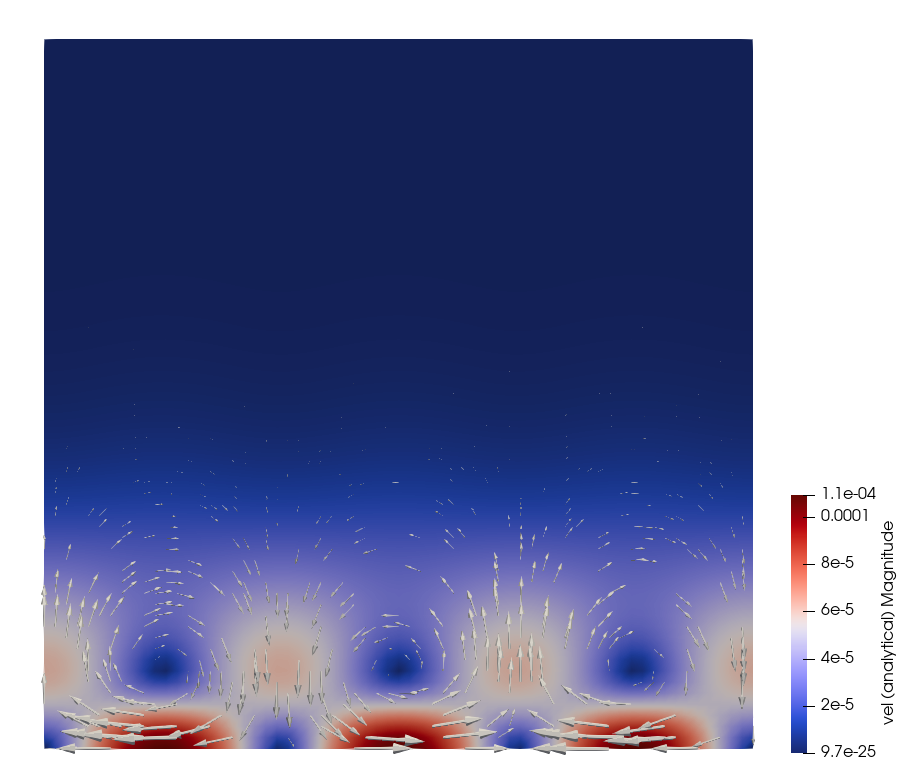
\includegraphics[width=5cm]{../images/fields/vel_solkz}
b)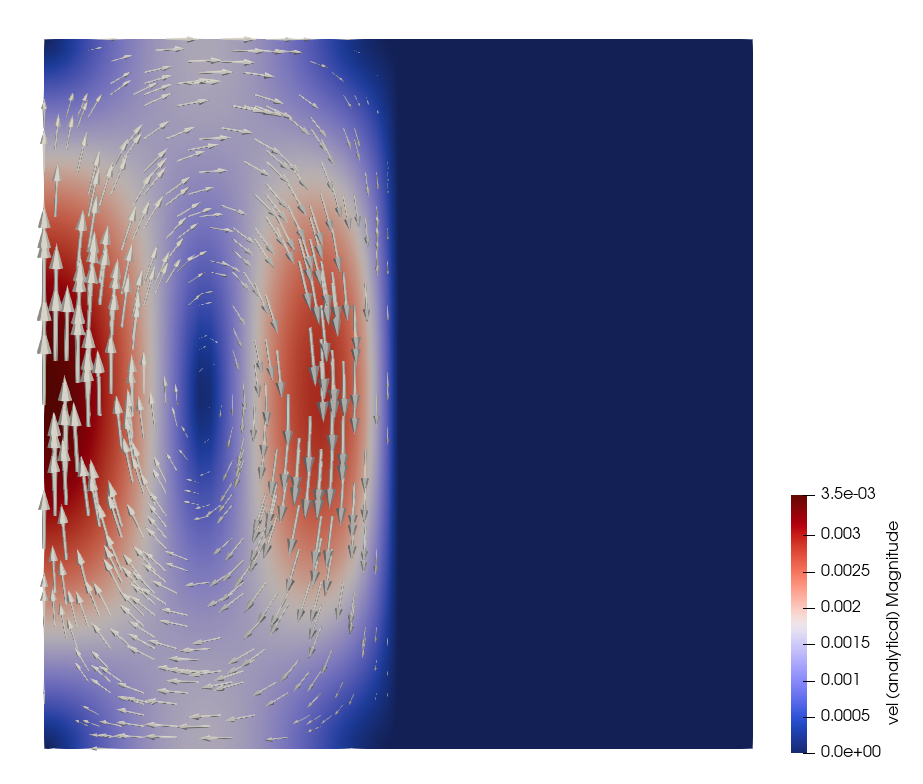
\includegraphics[width=5cm]{../images/fields/vel_solcx}\\
c)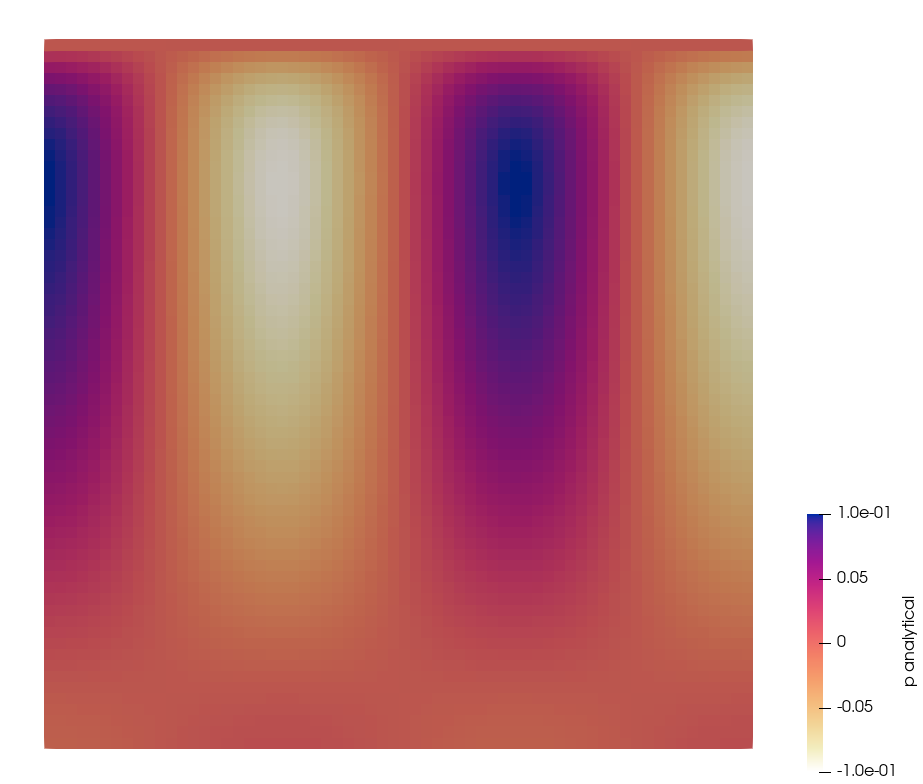
\includegraphics[width=5cm]{../images/fields/press_solkz}
d)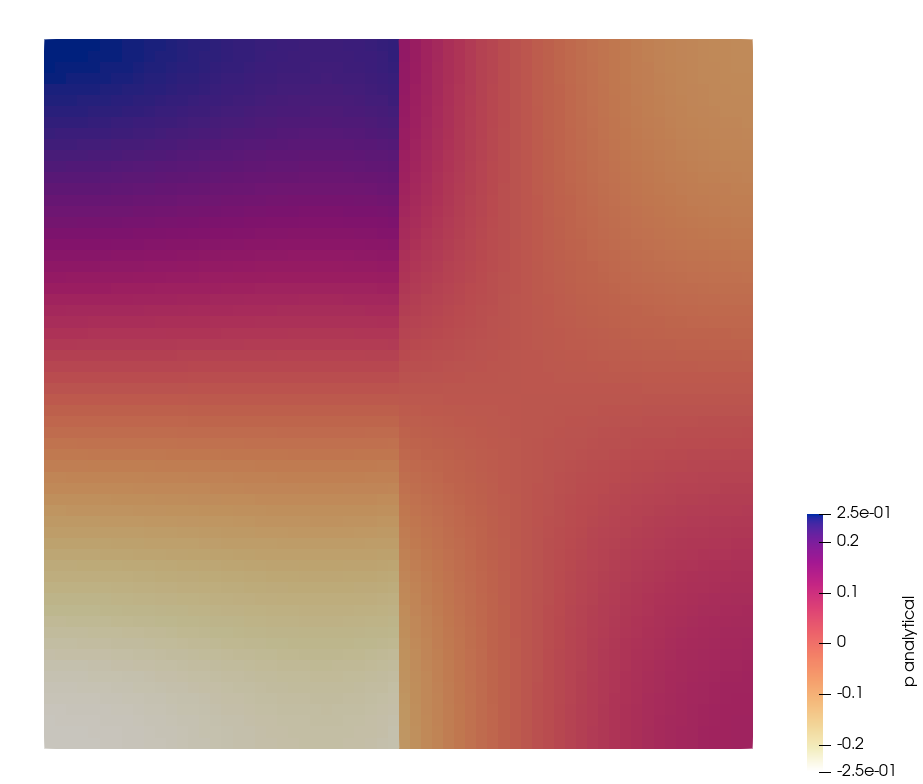
\includegraphics[width=5cm]{../images/fields/press_solcx}
\caption{Velocity and pressure fields for the SolKz (a,c) and SolCx (b,d) 
experiments.} \label{fig:sols}
\end{figure}

%experiment 5
For SolKz the viscosity is given by $\eta(y)=\exp(By)$ with $B=\ln 10^6 \simeq 13.8155$ 
and the density field by $\rho(x,y)=\sin(2y) \cos(3\pi x)$, with 
$\vec{g}=-\vec{e}_y$. 
Free slip boundary conditions are imposed on all sides of the domain.

\begin{figure}
\centering
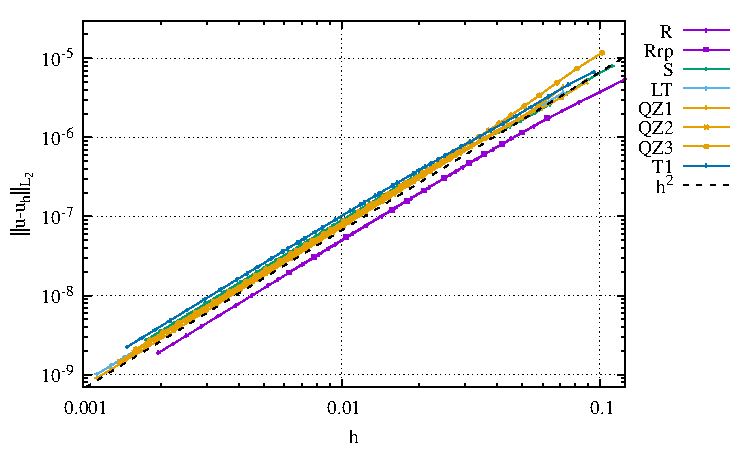
\includegraphics[width=8.9cm]{../results/errors_u_exp5}
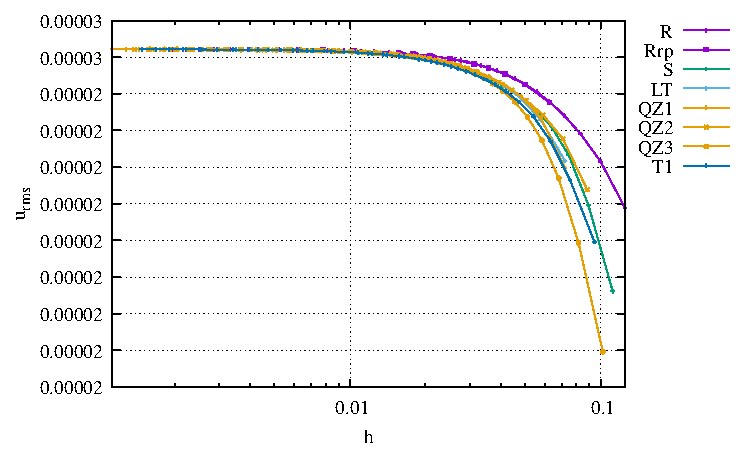
\includegraphics[width=8.9cm]{../results/vrms_exp5} \\
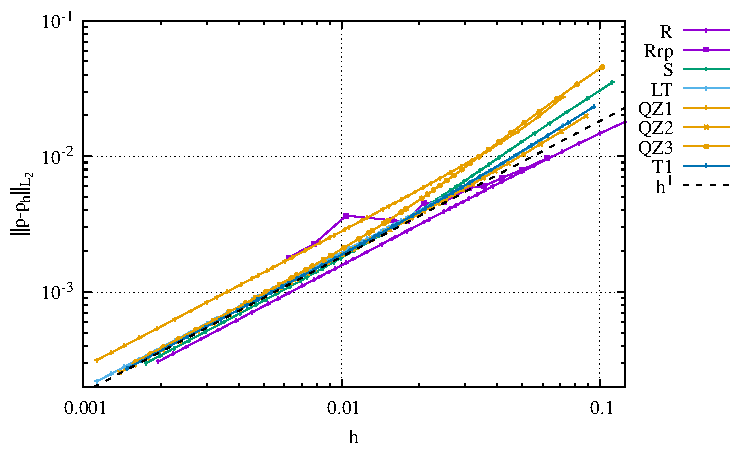
\includegraphics[width=8.9cm]{../results/errors_p_exp5}
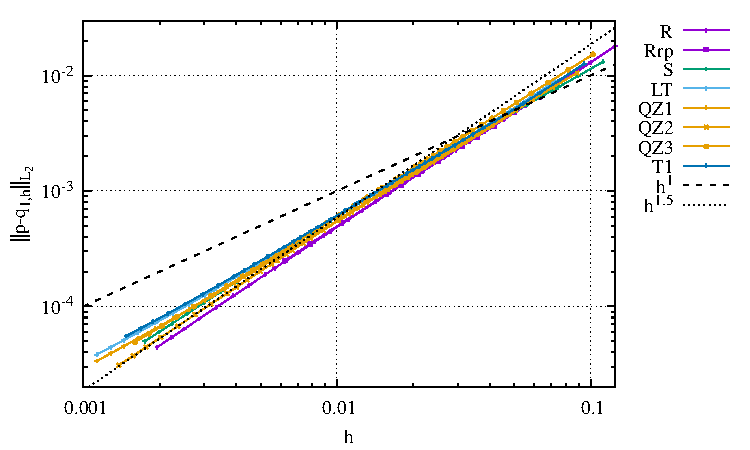
\includegraphics[width=8.9cm]{../results/errors_q1_exp5}
\caption{SolKz benchmark: velocity error, 
root mean square velocity, elemental pressure error and nodal pressure error
as a function of the mesh size $h$.} 
\label{fig:ressolkz}
\end{figure}

Discretization errors results are shown in Fig.~\ref{fig:ressolkz}.
Conclusions are nearly identical to those of the cavity benchmark:
all macro-element see their velocity error converge quadratically 
and their elemental pressure linearly, with R being the most accurate since 
no checkerboard modes are occuring.
Looking at the nodal pressure we see that S and QZ2 errors converge as $h^{1.5}$
while all others start with $h^{1.5}$ but ultimately end up $h^1$. 
{\color{red} actually it looks like it is about 1.45?? I need to rerun to highest resolution
and measure again}

%experiment 13
The second benchmark SolCx uses a discontinuous viscosity profile with a large jump in
the viscosity value along the middle of the domain ($\eta=1$ on the left,
$\eta=10^6$ on the right), resulting in a discontinuous pressure field. 
The domain is also a unit square, boundary conditions are free-slip on all edges, and
the gravity vector points downwards with $|{\bm g}| = 1$. 
The density is given by $\rho(x,y) = \sin(\pi y) \cos(\pi x)$.

Results are shown in Fig.~\ref{fig:ressolcx}.
Nodal pressure error rates are ommitted as all 
measured rates are $h^{0.5}$ since the averaging 
involves using elemental pressures on each side of the viscosity divide,
precisely where the analytical pressure is discontinuous.
All macro-element velocity errors converge quadratically 
while the pressure errors converge linearly.
Surprisingly pressure modes do not occur and the R macro-element
is the most accurate for both velocity {\it and} pressure.

\begin{figure}
\centering
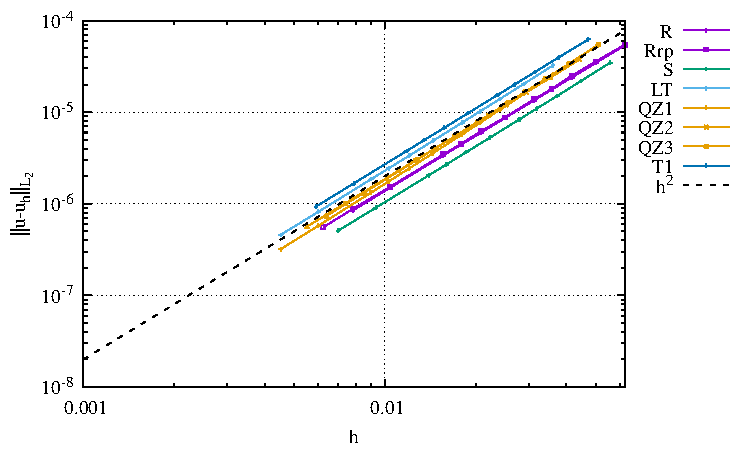
\includegraphics[width=8.9cm]{../results/errors_u_exp13}
%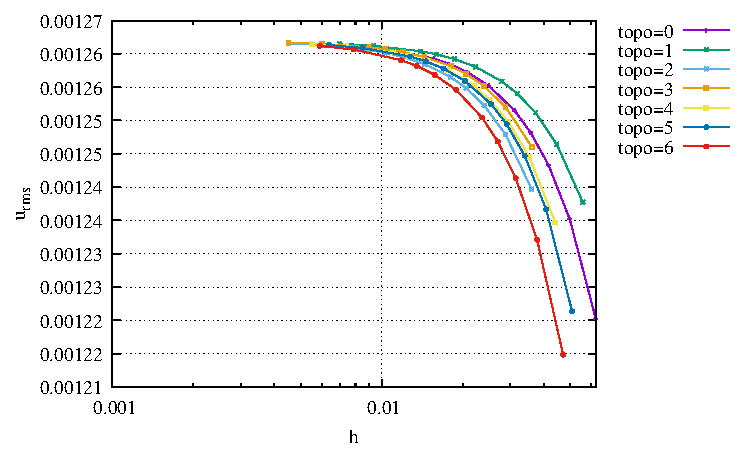
\includegraphics[width=8cm]{../results/vrms_exp13} \\
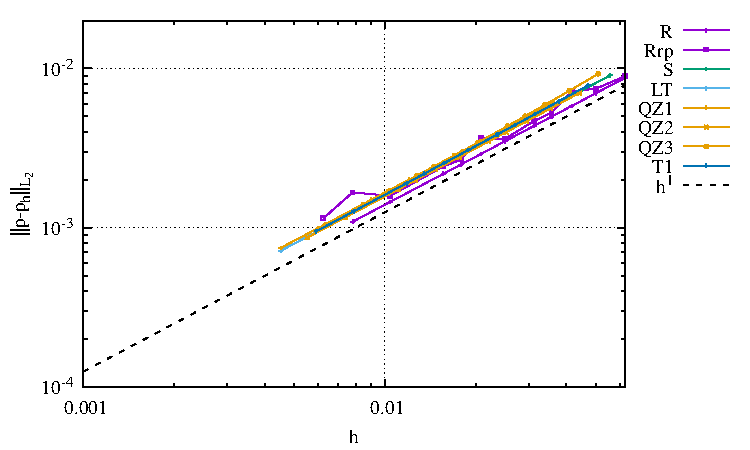
\includegraphics[width=8.9cm]{../results/errors_p_exp13}
%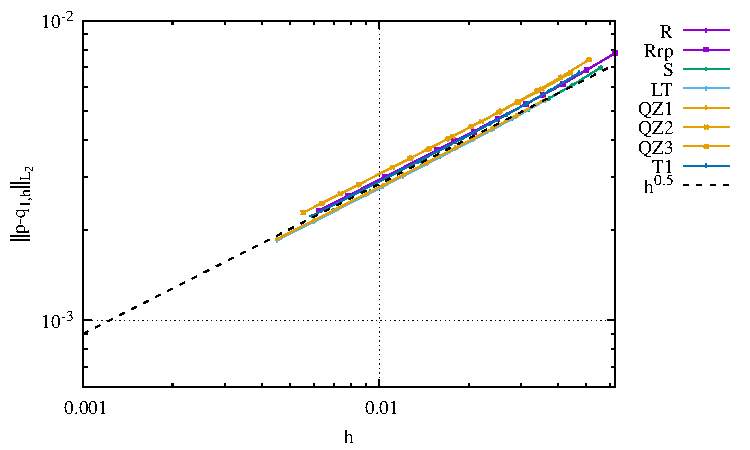
\includegraphics[width=8cm]{../results/errors_q1_exp13}
\caption{SolCx benchmark: velocity error, 
root mean square velocity, elemental pressure error and nodal pressure error
as a function of the the average mesh size $h$.
{\color{red} need to rerun it to high resolution}} 
\label{fig:ressolcx}
\end{figure}




%%%%%%%%%%%%%%%%%%%%%%%%%%%%%%%%%%%%%%%%%%%%%%%%%%%%%%%%%%
\section{Buoyancy-driven flow}



%paragraph for non geo ppl
What often characterizes geodynamical (mantle) modelling is the buoyancy-driven nature of the flow 
in the presence of a very strong hydrostatic pressure and a relatively small dynamic pressure.
On long periods of time the mantle and the lithosphere behave like non-Newtonian fluids
which effective viscosity ranges from about $10^{19}$ up to $10^{26}\si{\pascal\second}$, 
typical velocities are of the order of $1\si{\cm\per year}$, and pressure ranges from 
the atmospheric pressure at the surface ($\sim 10^5 \si{\pascal}$) up to about $100\si{\giga\pascal}$ 
at the core mantle boundary. The mantle is not well mixed and therefore not homeogenous: 
Subducted plate remnants which are colder than their surroundings are thought to slowly sink 
while thermo-chemical instabilities at the core mantle boundary are the location where 
so-called plumes root and traverse the mantle upwards.

The $Q_1\times P_0$ has been the workhorse of computational geodynamics for decades with 
very popular mantle convection and lithosphere deformation codes used in hundreds of publications
(see \cite{thba22} for a detailed list).
Note that it was also often employed with a pressure penalty formulation (\cite{kirh90,full95,brtf08}).

The following experiment is an idealized geodynamical setup
and is similar or even identical to the ones found in \cite{mamo08,gery10,thie11,sctc20,thba22,thba25}.
The 2d domain is a square of size $L_x=L_y=512$km filled with a fluid (the ``mantle'')
of density $\rho_1=3200\si{\kg\per\cubic\metre}$ 
and viscosity $\eta_1=10^{21}\si{\pascal\second}$.
A square block of size $128\times 128\si{\km}$ is placed in the domain and
is centered at location ($x_c,y_c$)=($256\si{\km}$, $384\si{\km}$) so 
as to insure that its edges
align with cell boundaries at all resolutions (we thereby wish to avoid
cases where the quadrature points inside an element would have different
density or viscosity associated to them). It is filled with a fluid
of density $\rho_2=\rho_1+\delta \rho$ and viscosity $\eta_2=\eta^\star \eta_1$.
The gravity vector points downwards with $|{\bm g}|=10\si{\metre\per\square\second}$. 
Boundary conditions are free slip on all sides.

Density variations are often small compared to the density of the mantle itself
and they can be positive or negative: in a geodynamical context, 
the block could be interpreted as a detached slab
($\delta\rho>0$) or a plume head ($\delta\rho<0$). 
We here choose $\delta \rho=+8\si{\kg\per\cubic\metre}$, i.e. $\delta \rho/\rho_1 = 0.25\%$.
This quantity was varied extensively in previous publications but as we will see 
this will not be needed in this case. 

%------------------------
\subsection{Full density}

This experiment was run for resolutions $16l\times 16l$ with $l=\{1,2,4,8\}$ and $\eta^\star=1$. 
We show in Fig.~\ref{fig:block1} the velocity field obtained for all meshes on 
a $16\times 16$ macro-element mesh. 
We find that {\it only} the R mesh yields a velocity field that is plausible, 
since all other 7 ones showcase very clear oscillations in and around the block.
We investigate further by analysing the vertical velocity $u_y$
on the line $x=L_x/2$ at different resolutions in Fig.~\ref{fig:block2}.
We find that with increasing resolution the oscillations decrease and 
all macro-elements converge to the expected velocity profile.


Finally, we also measure the pressure in the block 
at four locations corresponding to ($x_c \pm \delta x, y_c \pm \delta y$),
where $\delta x = \delta y = 0.1$ m, and show the normalized pressures
at all four of these locations in Fig.~\ref{fig:block3}.
{\color{red} describe}
This is in line with the results obtained by \cite{thba22} and 
all these observations lead us to conclude that 
macro-elements composed of $Q_1 \times P_0$ elements cannot be used for buoyancy 
driven flows unless (very) high resolutions are used.

\begin{figure}[t]
\centering
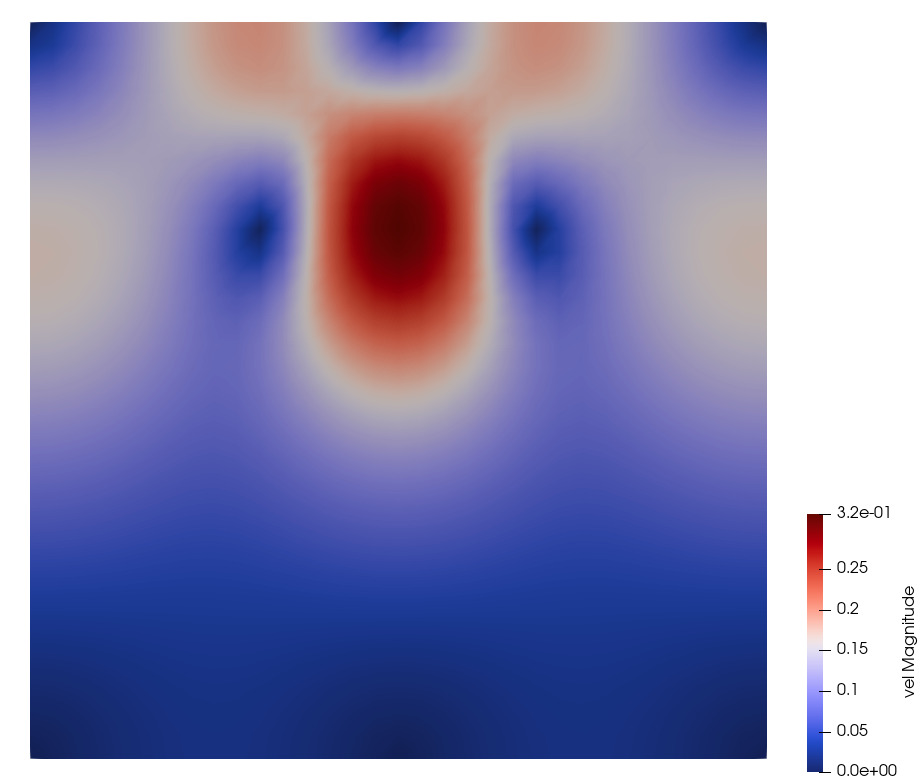
\includegraphics[width=4.3cm]{../results/exp08/fig16x16_full/vel0.jpg} % R
%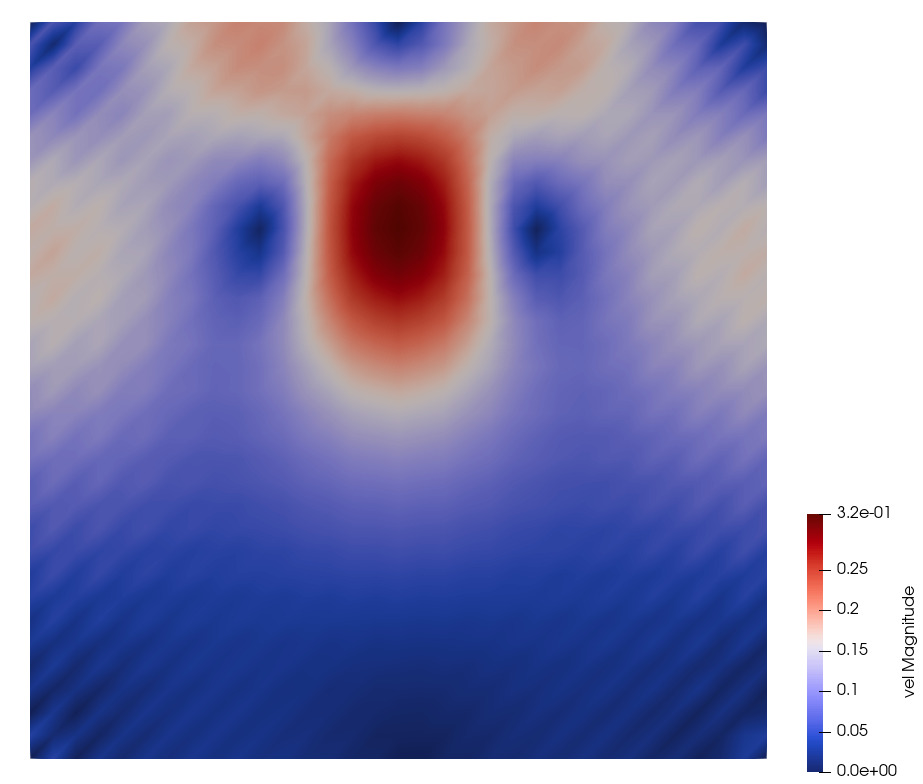
\includegraphics[width=4.3cm]{../results/exp08/fig16x16_full/vel8.png} % Rp
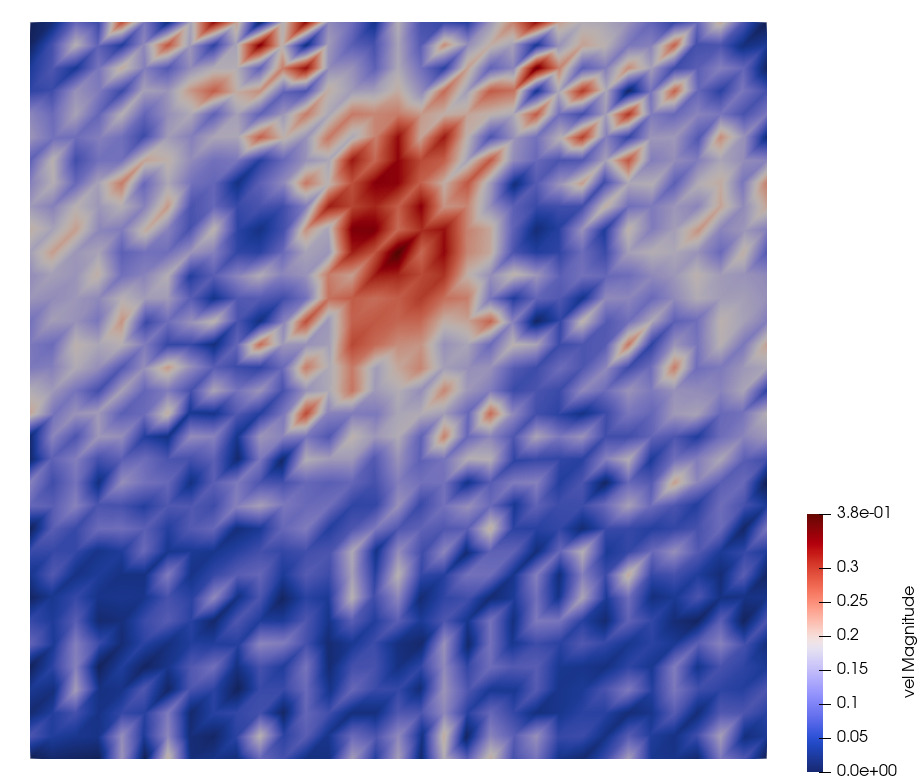
\includegraphics[width=4.3cm]{../results/exp08/fig16x16_full/vel9.jpg} % Rrp
%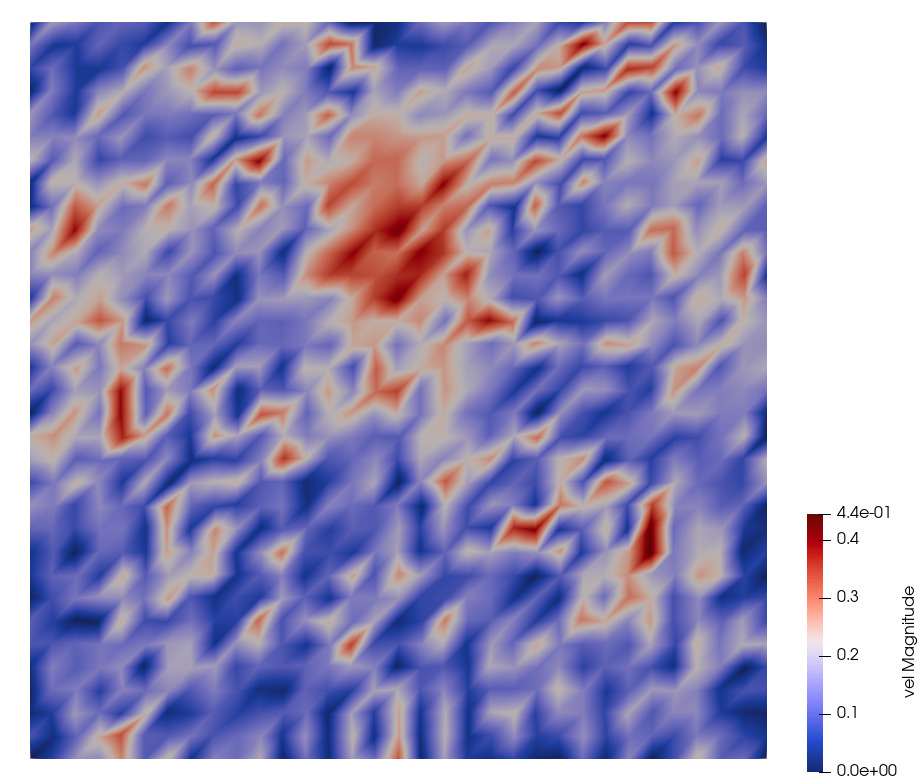
\includegraphics[width=4.3cm]{../results/exp08/fig16x16_full/vel10.png} % FR
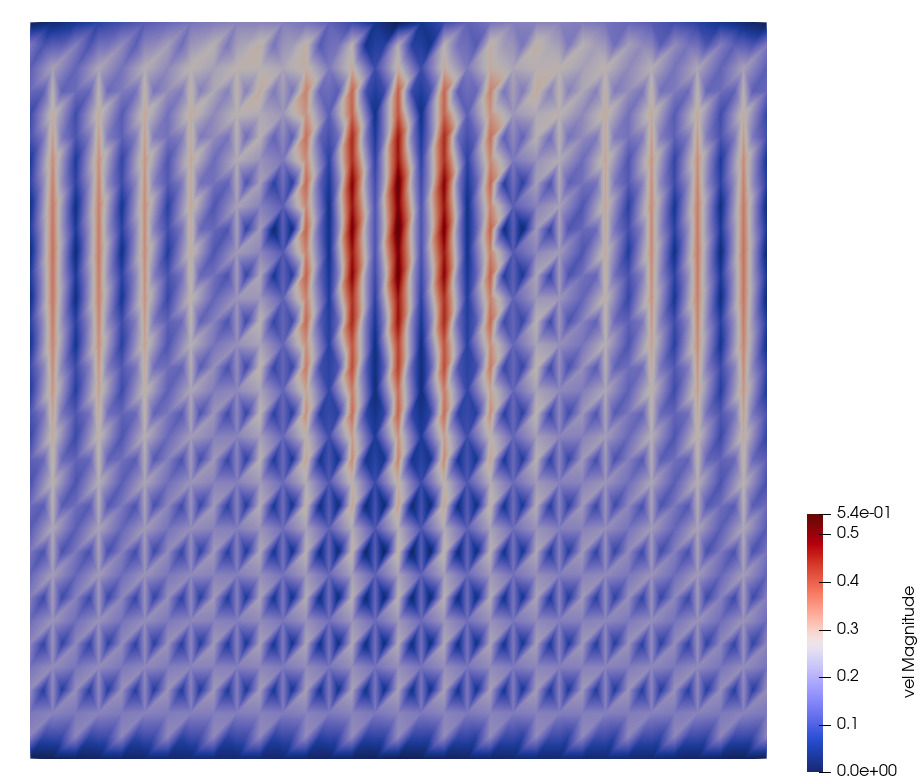
\includegraphics[width=4.3cm]{../results/exp08/fig16x16_full/vel1.jpg} %S
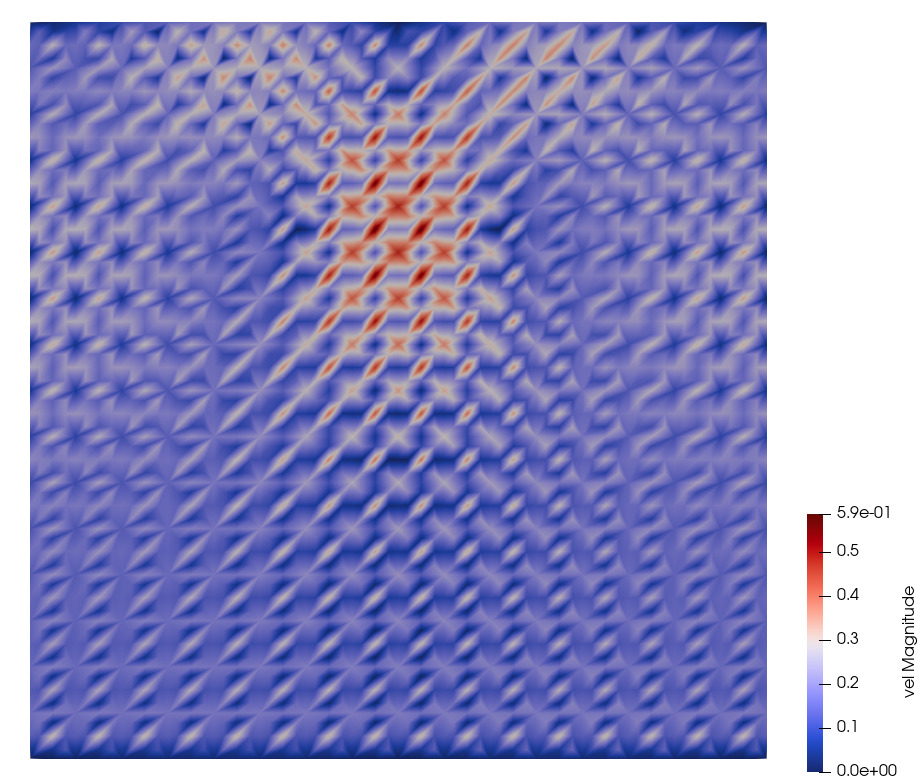
\includegraphics[width=4.3cm]{../results/exp08/fig16x16_full/vel2.jpg}\\ %LT
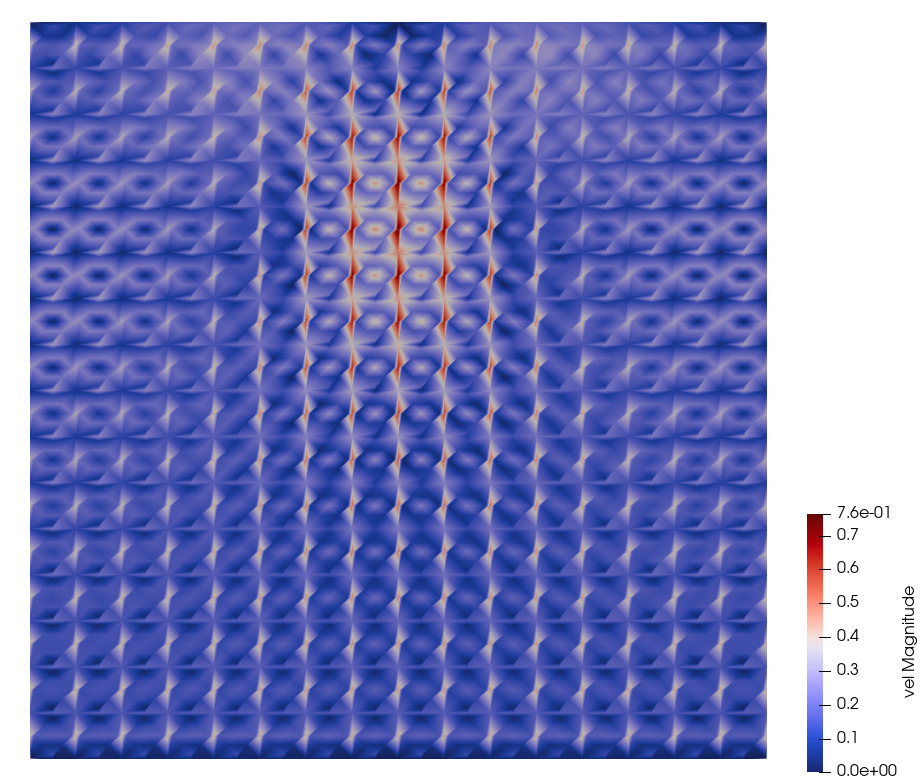
\includegraphics[width=4.3cm]{../results/exp08/fig16x16_full/vel3.jpg} %QZ1
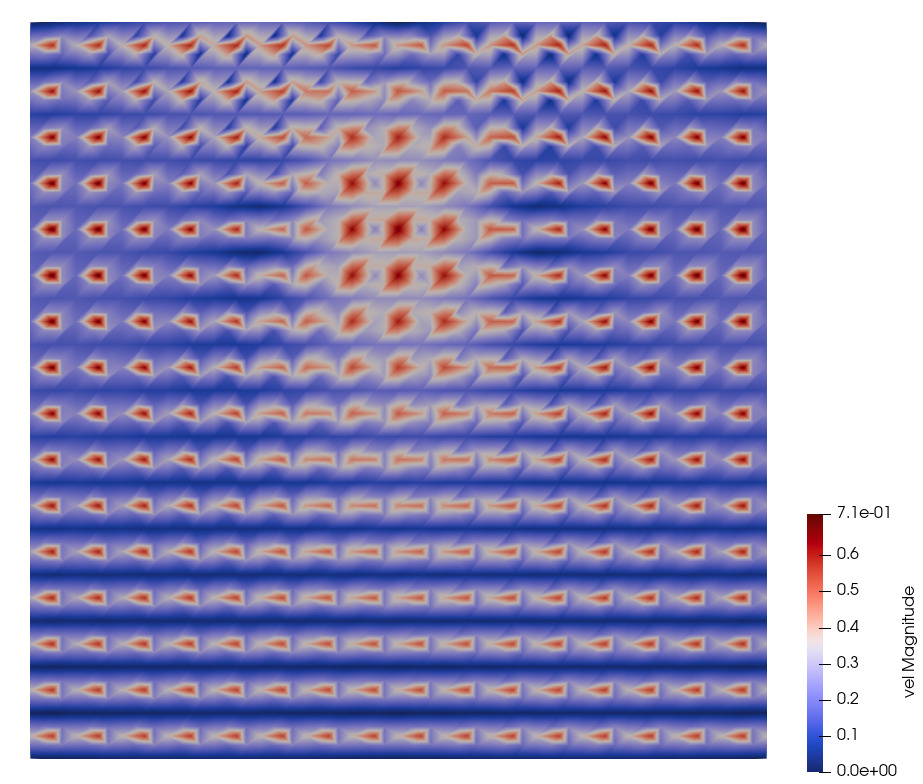
\includegraphics[width=4.3cm]{../results/exp08/fig16x16_full/vel4.jpg} %QZ2
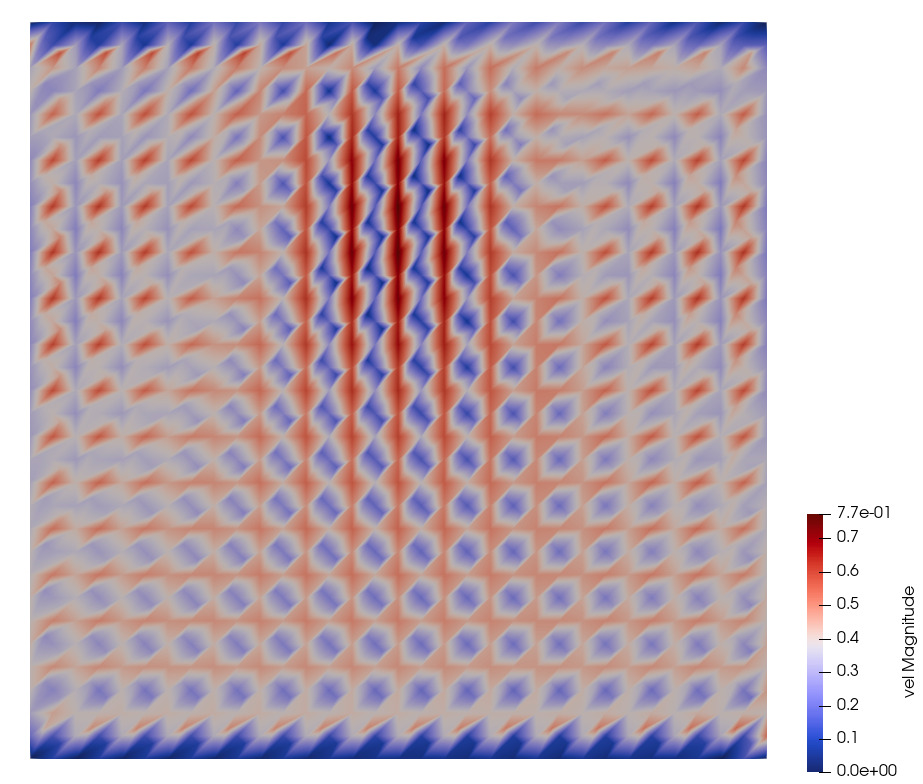
\includegraphics[width=4.3cm]{../results/exp08/fig16x16_full/vel5.jpg} %QZ3
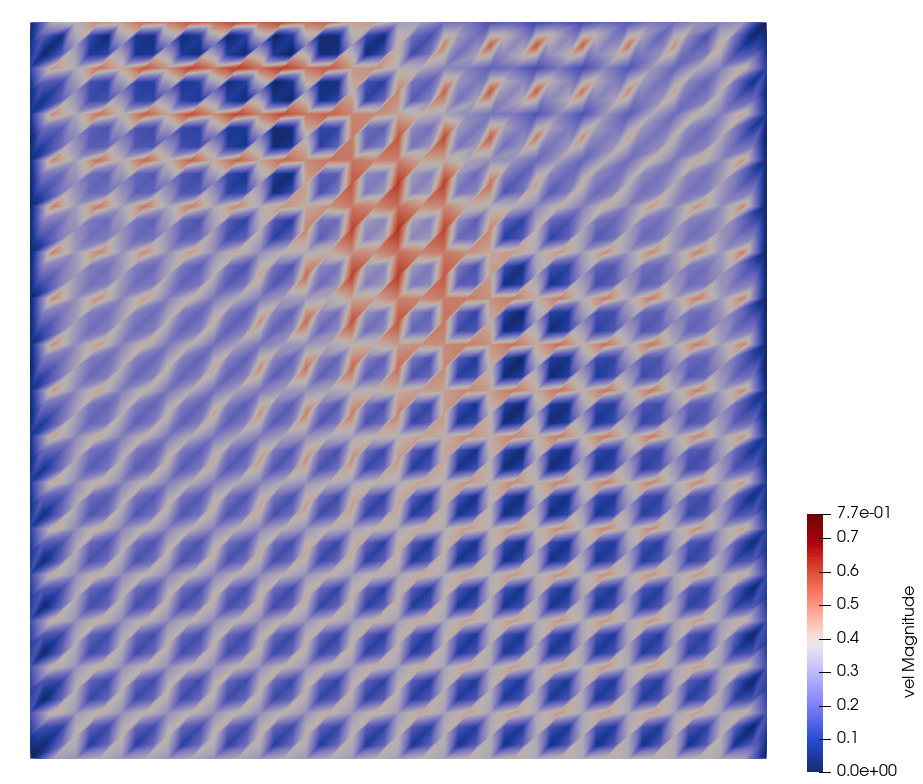
\includegraphics[width=4.3cm]{../results/exp08/fig16x16_full/vel6.jpg} % T1
%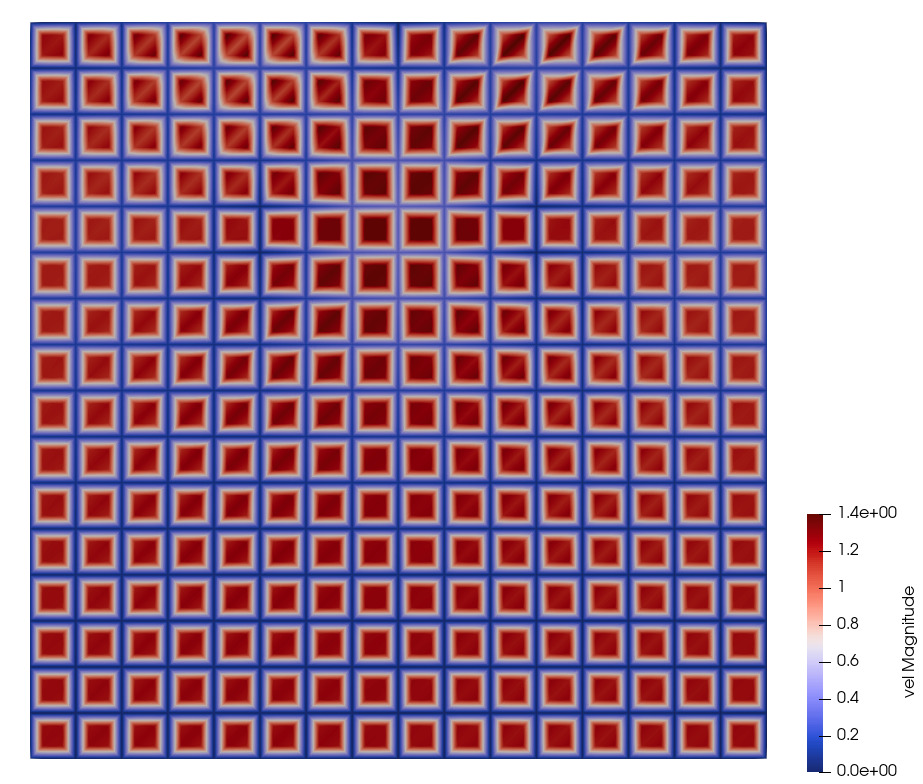
\includegraphics[width=4.3cm]{../results/exp08/fig16x16_full/vel7.png}
\caption{Sinking block experiment with full densities: velocity fields 
obtained with meshes composed of $16\times 16$ macro-elements.
From left to right, top to bottom: R, Rrp, S, LT, QZ1, QZ2, QZ3, T1.
The pressure fields need not be shown as they are visually dominated 
by the hydrostatic pressure.
\label{fig:block1}}
\end{figure}

\begin{figure}[t]
\centering
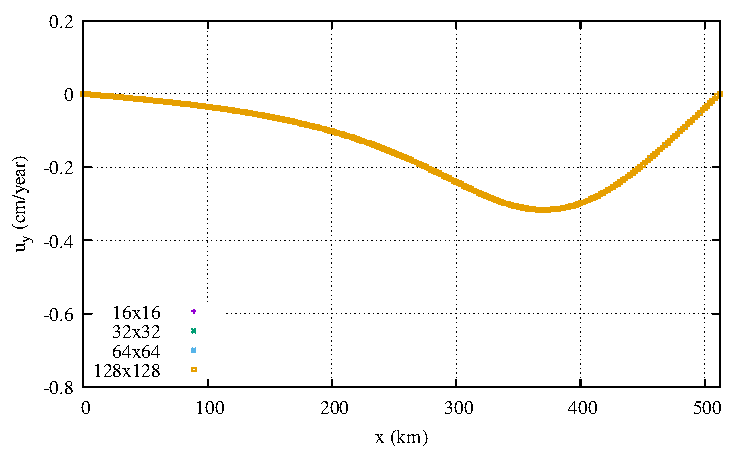
\includegraphics[width=5.8cm]{../results/exp08/vel_profile_topo0_full.pdf}
%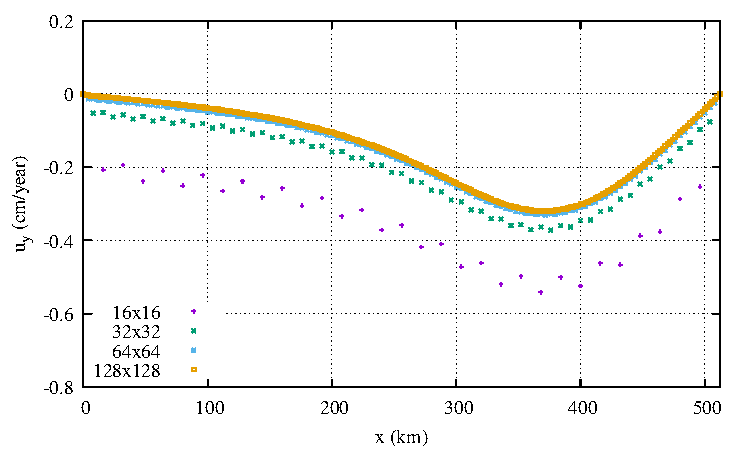
\includegraphics[width=4.3cm]{../results/exp08/vel_profile_topo1_full.pdf}
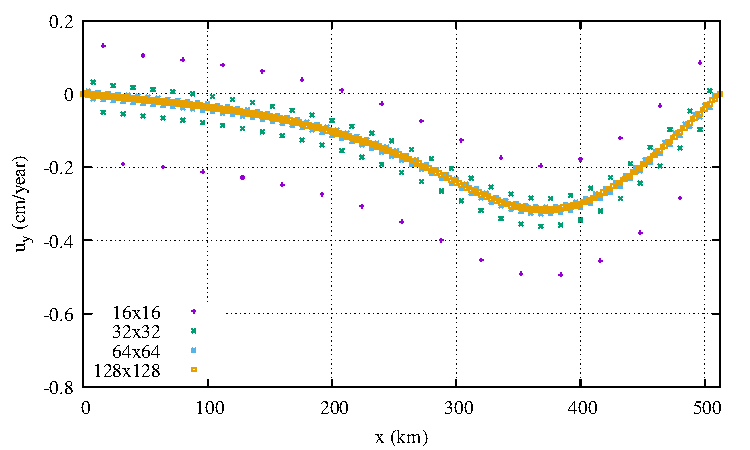
\includegraphics[width=5.8cm]{../results/exp08/vel_profile_topo2_full.pdf}
%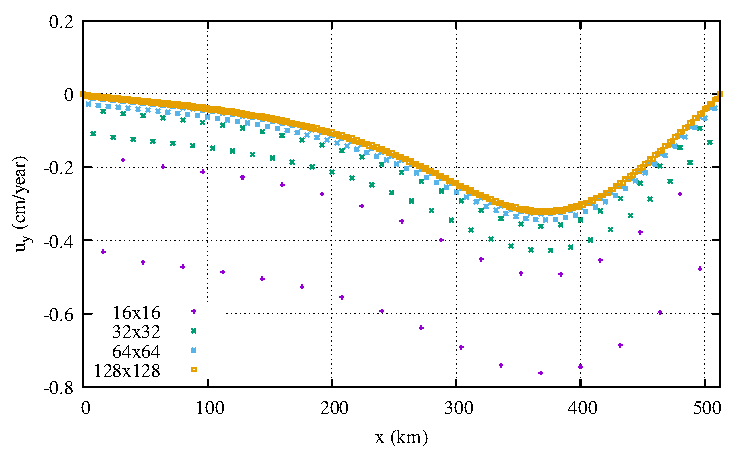
\includegraphics[width=4.3cm]{../results/exp08/vel_profile_topo3_full.pdf}\\
%\includegraphics[width=4.3cm]{../results/exp08/vel_profile_topo4_full.pdf}
%\includegraphics[width=4.3cm]{../results/exp08/vel_profile_topo5_full.pdf}
%\includegraphics[width=4.3cm]{../results/exp08/vel_profile_topo6_full.pdf}
%\includegraphics[width=4.3cm]{../results/exp08/vel_profile_topo7_full.pdf}\\
%\includegraphics[width=4.3cm]{../results/exp08/vel_profile_topo8_full.pdf}
\includegraphics[width=5.8cm]{../results/exp08/vel_profile_topo9_full.pdf}
%\includegraphics[width=4.3cm]{../results/exp08/vel_profile_topo10_full.pdf}
\caption{Sinking block experiment with full densities (isoviscous case): 
vertical velocity $u_y$ measured on the line $x=L_x/2$ passing through the middle of the block
for 4 different macro-element resolutions.
From left to right: R, LT, Rrp.
 \label{fig:block2}}
\end{figure}

\begin{figure}[t]
\centering
\includegraphics[width=8cm]{../results/exp08/p_block_res16.pdf}
\includegraphics[width=8cm]{../results/exp08/p_block_res32.pdf}\\
\includegraphics[width=8cm]{../results/exp08/p_block_res64.pdf}
\includegraphics[width=8cm]{../results/exp08/p_block_res128.pdf}
\caption{Sinking block experiment with full densities:  pressure in the middle
of the block for all meshes. Resolution 16x16 up to 128x128 macro-elements.  \label{fig:block3}}
\end{figure}


%------------------------
\subsection{Reduced density}

In an attempt to find a redeeming quality to the macro-elements 
we carry out an identical experiment albeit with so-called reduced densities:
the background lithostatic pressure is removed by substracting $\rho_1$
from all densities in the domain. In essence we are then solving for the dynamic
pressure alone. 
We find now that the velocity oscillations have disappeared 
so that all velocity fields visually resemble Fig.~\ref{fig:block1}a and 
there is no need present those. Instead we show the elemental pressure field in Fig.~\ref{fig:block4}.
Velocity profiles are also measured as in the full density case and 
all plots look identical to Fig.~\ref{fig:block2}a.

{\color{red} describe}

\begin{figure}[t]
\centering
\includegraphics[width=4.3cm]{../results/exp08/fig16x16_reduced/press.0000.png}
\includegraphics[width=4.3cm]{../results/exp08/fig16x16_reduced/press.0001.png}
\includegraphics[width=4.3cm]{../results/exp08/fig16x16_reduced/press.0002.png}
\includegraphics[width=4.3cm]{../results/exp08/fig16x16_reduced/press.0003.png}
\includegraphics[width=4.3cm]{../results/exp08/fig16x16_reduced/press.0004.png}
\includegraphics[width=4.3cm]{../results/exp08/fig16x16_reduced/press.0005.png}
\includegraphics[width=4.3cm]{../results/exp08/fig16x16_reduced/press.0006.png}
\includegraphics[width=4.3cm]{../results/exp08/fig16x16_reduced/press.0007.png}
\caption{Sinking block experiment with reduced densities: velocity fields 
obtained with meshes composed of $16\times 16$ macro-elements.
{\color{red} show q pressure?}
 \label{fig:block4}}
\end{figure}


{\color{red} not sure how much more in detail I should go wrt this.}





\newpage
%%%%%%%%%%%%%%%%%%%%%%%%%%%%%%%%%%%%%%%%%%%%%%%%%%%%%%%%%%%%%%%%%%%
\section{Conclusions}\label{sec5}

\begin{itemize}
\item Conclusions about manufactured solutions:\\
R nearly always better for velocity but pressure modes amplitude unpredictable.
S often best stable m-e, followed by QZ2.

\item Conclusions about buoyancy-driven flows\\
use in geodynamics possible IF reduced density or rather high resolution (but then why not Q2xQ1). 
S is probably best overal.

\item
{\color{blue} W: macro-e have two advantages: no checkerboard modes {\it and} LBB stable. 
So CG applied to Schur complement should converge in a number of iterations independent of $h$.
Should I explore this, plug in my citcom like solver (precond CG on Schur complement)
and look at which m-e requires the least iterations? it is some work, but if you think
it is valuable, happy to do it :)}

\item 
Thoughts about use of m-e in comp geodynamics: 
somewhat awkward with particle-in-cell. inner structure of macro-element could influence shear band angle. 
What about annulus, or mesh deformation bc of ALE?

\item T1 seems stable. I compute the null space size for this macro-element in appendix B
and it seems to be 1. Since its accuracy is low, no need to formally prove its stability?
 
\item can we extend all/some to 3D? stability proof ? I am not aware of any m-e in 3d !?
really, I just can't find a single paper with m-e similar to the ones above in 3d

\end{itemize}



%compute indicator (eigenvalue, ... ?) for meshes and rank them ? see chappelle bathe

%I need to understand how to prove LBB stability and apply it to 3D elts ?

%I disregard randomised regular meshes bc how much random is not clear.


\printbibliography

\appendix

\section{Relationship between QZ1 and QZ3}



\begin{center}
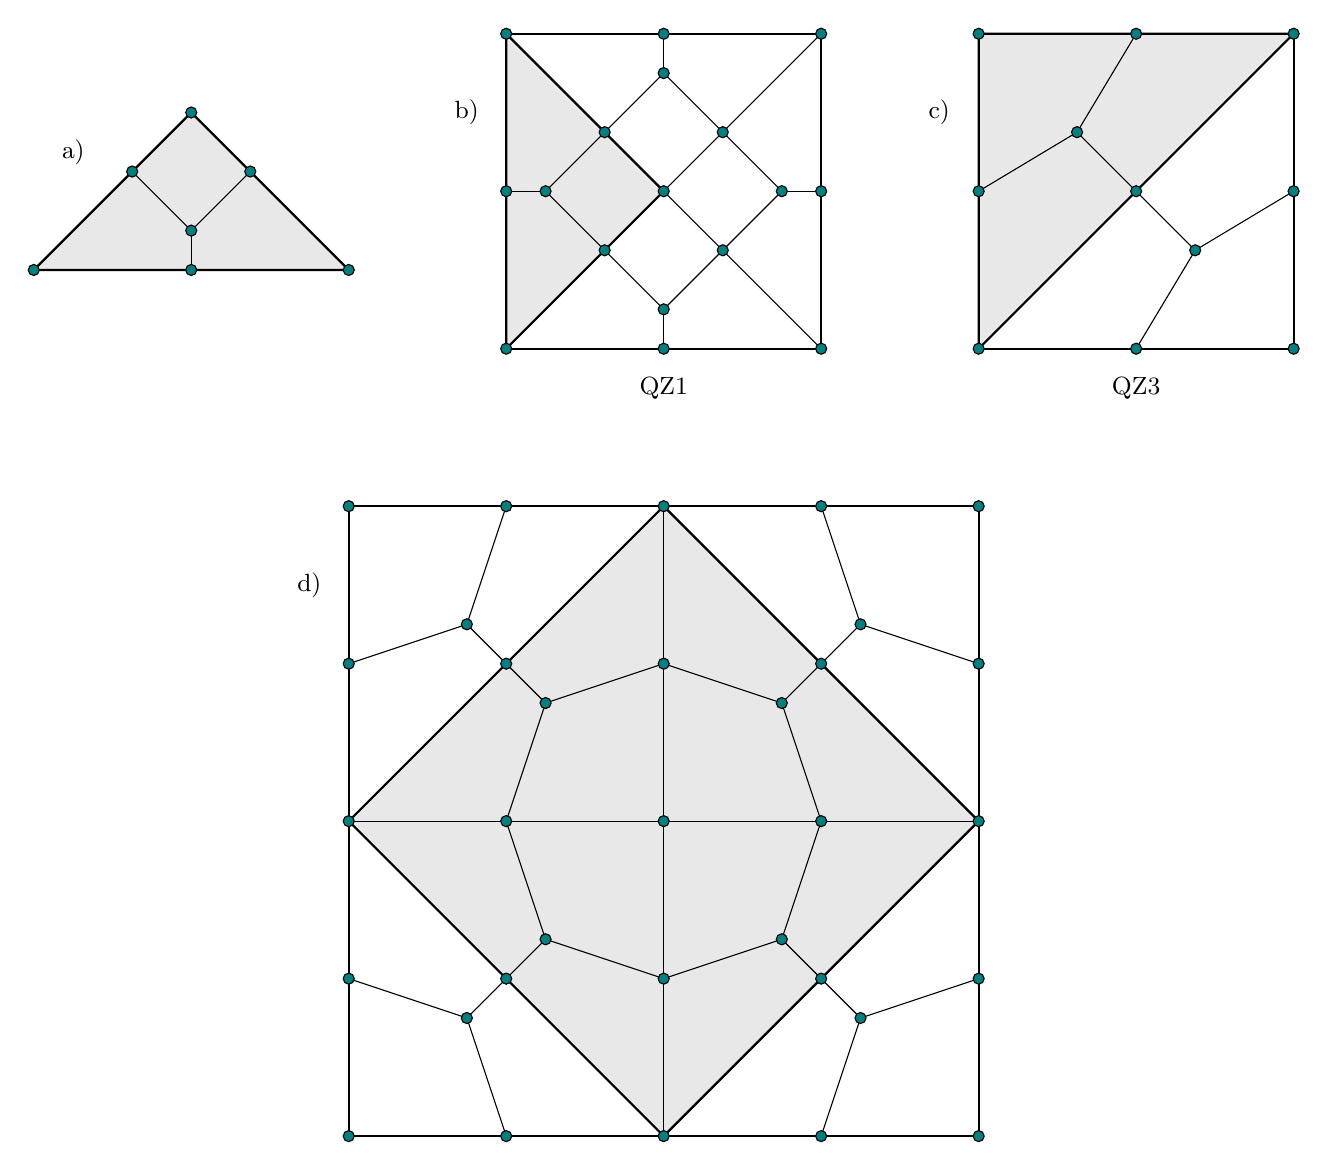
\begin{tikzpicture}
%\draw[fill=gray!13,gray!13](0,0) rectangle (16,16);
%\draw[step=0.5cm,gray,very thin] (0,0) grid (16,16); %background grid

%triangle
\draw[thick,fill=gray!18] (0,12)--(4,12)--(2,14)--cycle;
\draw[] (2,12)--(2,12.5);
\draw[] (2,12.5)--(1.25,13.25);
\draw[] (2,12.5)--(2.75,13.25);

\draw[black,fill=teal] (0,12)   circle (2pt);
\draw[black,fill=teal] (4,12)   circle (2pt);
\draw[black,fill=teal] (2,14)   circle (2pt);
\draw[black,fill=teal] (2,12)   circle (2pt);
\draw[black,fill=teal] (2,12.5)   circle (2pt);
\draw[black,fill=teal] (1.25,13.25)   circle (2pt);
\draw[black,fill=teal] (2.75,13.25)   circle (2pt);


% QZ1
\draw[thick,fill=gray!18] (6,11)--(8,13)--(6,15)--cycle;
\draw[thick] (6,11)--(10,11)--(10,15)--(6,15)--cycle;
\draw[] (6,11)--(10,15);
\draw[] (6,15)--(10,11);
\draw[] (6.5,13)--(8,11.5)--(9.5,13)--(8,14.5)--cycle;
\draw[] (6,13)--(6.5,13);
\draw[] (9.5,13)--(10,13);
\draw[] (8,11)--(8,11.5);
\draw[] (8,14.5)--(8,15);

\draw[black,fill=teal] (6,11)   circle (2pt);
\draw[black,fill=teal] (8,11)   circle (2pt);
\draw[black,fill=teal] (10,11)   circle (2pt);
\draw[black,fill=teal] (6,13)   circle (2pt);
\draw[black,fill=teal] (8,13)   circle (2pt);
\draw[black,fill=teal] (10,13)   circle (2pt);
\draw[black,fill=teal] (6,15)   circle (2pt);
\draw[black,fill=teal] (8,15)   circle (2pt);
\draw[black,fill=teal] (10,15)   circle (2pt);
\draw[black,fill=teal] (6.5,13)   circle (2pt);
\draw[black,fill=teal] (8,11.5)   circle (2pt);
\draw[black,fill=teal] (9.5,13)   circle (2pt);
\draw[black,fill=teal] (8,14.5)   circle (2pt);
\draw[black,fill=teal] (8.75,13.75)   circle (2pt);
\draw[black,fill=teal] (7.25,13.75)   circle (2pt);
\draw[black,fill=teal] (8.75,12.25)   circle (2pt);
\draw[black,fill=teal] (7.25,12.25)   circle (2pt);

% QZ3 %%%%%%%%%%%%%%%%%%%%%%%%%%%%%%%%%%%%%%%%%%%%%%%%%%%%%%%%%%%%%

\draw[thick,fill=gray!18] (12,11)--(16,15)--(12,15)--cycle;

\draw[thick] (12,11)--(16,11)--(16,15)--(12,15)--cycle;
\draw[] (12,11)--(16,15);
\draw[] (12,13)--(13.25,13.75)--(14,15);
\draw[] (14,11)--(14.75,12.25)--(16,13);
\draw[] (13.25,13.75)--(14.75,12.25);

\draw[black,fill=teal] (12,11)   circle (2pt);
\draw[black,fill=teal] (14,11)   circle (2pt);
\draw[black,fill=teal] (16,11)   circle (2pt);
\draw[black,fill=teal] (12,13)   circle (2pt);
\draw[black,fill=teal] (14,13)   circle (2pt);
\draw[black,fill=teal] (16,13)   circle (2pt);
\draw[black,fill=teal] (12,15)   circle (2pt);
\draw[black,fill=teal] (14,15)   circle (2pt);
\draw[black,fill=teal] (16,15)   circle (2pt);
\draw[black,fill=teal] (13.25,13.75)   circle (2pt);
\draw[black,fill=teal] (14.75,12.25)   circle (2pt);


% big %%%%%%%%%%%%%%%%%%%%%%%%%%%%%%%%%%%%%%%%%%%%%%%%%%%%%%%%

\draw[thick,fill=gray!18] (8,1)--(12,5)--(8,9)--(4,5)--cycle;
\draw[thick] (4,1)--(12,1)--(12,9)--(4,9)--cycle;
\draw[] (4,5)--(12,5);
\draw[] (8,1)--(8,9);
\draw[] (8,1)--(12,5)--(8,9)--(4,5)--cycle;
\draw[] (5.5,2.5)--(6.5,3.5);
\draw[] (4,3)--(5.5,2.5)--(6,1);
\draw[] (9.5,3.5)--(10.5,2.5);
\draw[] (10,1)--(10.5,2.5)--(12,3);
\draw[] (9.5,6.5)--(10.5,7.5);
\draw[] (12,7)--(10.5,7.5)--(10,9);
\draw[] (5.5,7.5)--(6.5,6.5);
\draw[] (4,7)--(5.5,7.5)--(6,9);
\draw[] (6,5)--(6.5,6.5)--(8,7)--(9.5,6.5)--(10,5)--(9.5,3.5)--(8,3)--(6.5,3.5)--cycle;

%\draw[thick,->] (0.75,1) -- (9,1)  ;
%\draw[thin, dashed] (1,1.25) -- (2.5,1.25)  ;
\node[] at (0.5,13.5) {\small a)};
\node[] at (5.5,14) {\small b)}; \node[] at (8,10.5) {\small QZ1};
\node[] at (11.5,14) {\small c)}; \node[] at (14,10.5) {\small QZ3};
\node[] at (3.5,8) {\small d)};

\draw[black,fill=teal] (4,1)   circle (2pt);
\draw[black,fill=teal] (6,1)   circle (2pt);
\draw[black,fill=teal] (8,1)   circle (2pt);
\draw[black,fill=teal] (10,1)   circle (2pt);
\draw[black,fill=teal] (12,1)   circle (2pt);
\draw[black,fill=teal] (4,3)   circle (2pt);
\draw[black,fill=teal] (6,3)   circle (2pt);
\draw[black,fill=teal] (8,3)   circle (2pt);
\draw[black,fill=teal] (10,3)   circle (2pt);
\draw[black,fill=teal] (12,3)   circle (2pt);
\draw[black,fill=teal] (4,5)   circle (2pt);
\draw[black,fill=teal] (6,5)   circle (2pt);
\draw[black,fill=teal] (8,5)   circle (2pt);
\draw[black,fill=teal] (10,5)   circle (2pt);
\draw[black,fill=teal] (12,5)   circle (2pt);
\draw[black,fill=teal] (4,7)   circle (2pt);
\draw[black,fill=teal] (6,7)   circle (2pt);
\draw[black,fill=teal] (8,7)   circle (2pt);
\draw[black,fill=teal] (10,7)   circle (2pt);
\draw[black,fill=teal] (12,7)   circle (2pt);
\draw[black,fill=teal] (4,9)   circle (2pt);
\draw[black,fill=teal] (6,9)   circle (2pt);
\draw[black,fill=teal] (8,9)   circle (2pt);
\draw[black,fill=teal] (10,9)   circle (2pt);
\draw[black,fill=teal] (12,9)   circle (2pt);

\draw[black,fill=teal] (5.5,2.5)   circle (2pt);
\draw[black,fill=teal] (10.5,2.5)   circle (2pt);
\draw[black,fill=teal] (5.5,7.5)   circle (2pt);
\draw[black,fill=teal] (10.5,7.5)   circle (2pt);

\draw[black,fill=teal] (6.5,3.5)   circle (2pt);
\draw[black,fill=teal] (9.5,3.5)   circle (2pt);
\draw[black,fill=teal] (6.5,6.5)   circle (2pt);
\draw[black,fill=teal] (9.5,6.5)   circle (2pt);


\end{tikzpicture}
\end{center}






a) triangle subdivided into three quadrilateral elements.
b) QZ1 macro-element. The greyed area shows that this macro-element is 
in fact composed of four triangles similar to a).
c) QZ3 macro-element. The greyed area shows that this macro-element is
in fact composed of two triangles similar to a).
d) Four QZ3 macro-elements (two with a SW-NE diagonal, two with a NW-SE diagonal).
The greyed area highlights the presence of a QZ1 macro-element. 


\newpage
\section{About nullspaces}



The nullspace of the ${ \bm G}$ operator can be determined 
numerically (at least for small enough meshes). 
It is first built with a size $NfemV \times NfemP$.
In a second time the lines corresponding to degrees of freedom 
where a Dirichlet boundary condition is applied are removed to yield
the $\tilde{\bm G}$ matrix. 

The null space of $\tilde{\bm G}$ is then obtained with the 
{\tt null\_space} function from {\tt scipy.linalg}.
I report below the size of the null space for all 11 topologies/meshes
and for meshes consisting of $1\times 1$ macro-element up to $10\times 10$.

As explained (for example) in \cite{sagl81a}, if an element is stable we 
expect the size of the null space to be one, corresponding to the 
hydrostatic pressure mode.
We find that the R mesh null space is always two, thereby confirming 
the presence of a checkerboard pressure mode at all resolutions. 
The S, LT, QZ1, QZ2, QZ3 null spaces are unsurprisingly of size 1 since 
these macro-elements have been proven LBB stable. 
The T1 null space size is also always 1 which indicates that it could be stable,
while T2 null space size is always 2 for 2x2 and higher meshes.
Finally the Rp, Rrp and FR meshes all yield null spaces of size 1 
provided that at least a 3x3 macro-element is used which is very much the 
case in practice. 

\begin{center}
\includegraphics[width=14cm]{../results/nullspace/nullspace_NS.pdf}\\
No-slip on all sides
\end{center}


%\begin{center}
%\includegraphics[width=10cm]{../results/nullspace/nullspace_FS.pdf}\\
%Free-slip on all sides
%\end{center}


%%%%%%%%%%%%%%%%%%%%%%%%%%%%%%%%%%%%%%%%%%%%%%%%%%%%%%%%%%%%%%%
\section{About the macro-element internal geometry}

{\color{red} this is a very rough appendix -- needs to be revisited/finished}
In what follows I find out which macro-element 
can be built of equal area elements and compute 
the corresponding $\epsilon$ parameter which controls the positioning of the internal nodes.

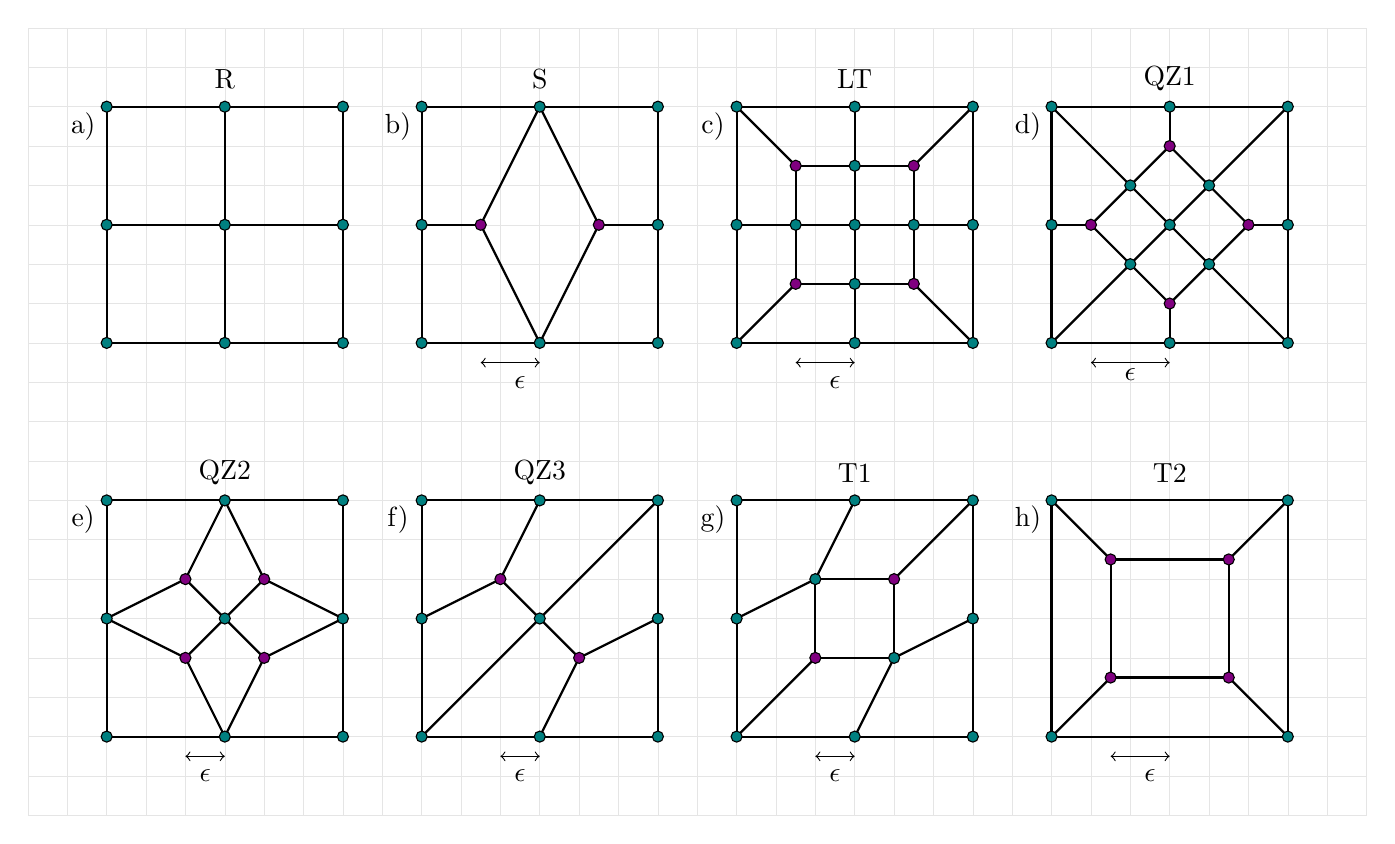
\begin{tikzpicture}
%\draw[fill=gray!23,gray!23](0,0) rectangle (5,5);
\draw[step=0.5cm,gray!20,very thin] (0,0) grid (17,10); %background grid

%%%%%%%%%%%%%%%%%%%%%%%%%%%%%%%%%%%%%%%%%%%%%%%%%%%%%%%%%%
\node[] at (0.7,3.75) {e)};
\draw[thick] (1,1) -- (4,1) -- (4,4) -- (1,4) -- cycle;  

\draw[thick] (1,2.5)--(2,3)--(2.5,4)--(3,3)--(4,2.5)--(3,2)--(2.5,1)--(2,2)--cycle;
\draw[thick] (2,2)--(3,3);
\draw[thick] (2,3)--(3,2);

\draw[black,fill=teal] (1,1)   circle (2pt);
\draw[black,fill=teal] (1,4)   circle (2pt);
\draw[black,fill=teal] (4,1)   circle (2pt);
\draw[black,fill=teal] (4,4)   circle (2pt);
\draw[black,fill=teal] (2.5,2.5)   circle (2pt);

\draw[black,fill=teal] (1,2.5)   circle (2pt);
\draw[black,fill=teal] (4,2.5)   circle (2pt);
\draw[black,fill=teal] (2.5,1)   circle (2pt);
\draw[black,fill=teal] (2.5,4)   circle (2pt);

\draw[black,fill=violet] (2,2)   circle (2pt);
\draw[black,fill=violet] (3,2)   circle (2pt);
\draw[black,fill=violet] (2,3)   circle (2pt);
\draw[black,fill=violet] (3,3)   circle (2pt);

\draw[<->] (2,0.75)--(2.5,0.75); \node[] at (2.25,0.5) {$\epsilon$};

\node[] at (2.5,4.35) {QZ2};

%%%%%%%%%%%%%%%%%%%%%%%%%%%%%%%%%%%%%%%%%%%%%%%%%%%%%%%%%%%%%
\node[] at (4.7,3.75) {f)};
\draw[thick] (5,1) -- (8,1) -- (8,4) -- (5,4) -- cycle;  


\draw[thick] (6.5,1)--(7,2)--(8,2.5) ; 
\draw[thick] (5,2.5)--(6,3)--(6.5,4) ; 
\draw[thick] (6,3)--(7,2);
\draw[thick] (5,1)--(8,4);

\draw[black,fill=teal] (5,1)   circle (2pt);
\draw[black,fill=teal] (5,4)   circle (2pt);
\draw[black,fill=teal] (8,1)   circle (2pt);
\draw[black,fill=teal] (8,4)   circle (2pt);
\draw[black,fill=teal] (6.5,2.5)  circle (2pt);
\draw[black,fill=teal] (5,2.5)   circle (2pt);
\draw[black,fill=teal] (8,2.5)   circle (2pt);
\draw[black,fill=teal] (6.5,1)   circle (2pt);
\draw[black,fill=teal] (6.5,4)   circle (2pt);

\draw[black,fill=violet] (6,3)   circle (2pt);
\draw[black,fill=violet] (7,2)   circle (2pt);


\draw[<->] (6,0.75)--(6.5,0.75); \node[] at (6.25,0.5) {$\epsilon$};

\node[] at (6.5,4.35) {QZ3};

%%%%%%%%%%%%%%%%%%%%%%%%%%%%%%%%%%%%%%%%%%%%%%%%%%%%%%%%%%%%%
\node[] at (8.7,3.75) {g)};
\draw[thick] (9,1) -- (12,1) -- (12,4) -- (9,4) -- cycle;  
\draw[thick] (10,2)--(11,2)--(11,3)--(10,3)--cycle; 
\draw[thick] (9,1)--(10,2);
\draw[thick] (11,3)--(12,4);
\draw[thick] (10.5,1)--(11,2)--(12,2.5);
\draw[thick] (9,2.5)--(10,3)--(10.5,4);

\draw[black,fill=teal] (9,1)   circle (2pt);
\draw[black,fill=teal] (10.5,1)   circle (2pt);
\draw[black,fill=teal] (12,1)   circle (2pt);
\draw[black,fill=teal] (9,2.5)   circle (2pt);
\draw[black,fill=teal] (12,2.5)   circle (2pt);
\draw[black,fill=teal] (9,4)   circle (2pt);
\draw[black,fill=teal] (10.5,4)   circle (2pt);
\draw[black,fill=teal] (12,4)   circle (2pt);
\draw[black,fill=teal] (10,3)   circle (2pt);
\draw[black,fill=teal] (11,2)   circle (2pt);

\draw[black,fill=violet] (10,2)   circle (2pt);
\draw[black,fill=violet] (11,3)   circle (2pt);


\draw[<->] (10,0.75)--(10.5,0.75); \node[] at (10.25,0.5) {$\epsilon$};

\node[] at (10.5,4.35) {T1};


%%%%%%%%%%%%%%%%%%%%%%%%%%%%%%%%%%%%%%%%%%%%%%%%%%%%%%%%%%%
\node[] at (12.7,3.75) {h)};
\draw[thick] (13,1) -- (16,1) -- (16,4) -- (13,4) -- cycle;  


\draw[thick] (13.75,1.75)--(15.25,1.75)--(15.25,3.25)--(13.75,3.25)--cycle; 
\draw[thick] (13,1)--(13.75,1.75); 
\draw[thick] (16,1)--(15.25,1.75); 
\draw[thick] (13,4)--(13.75,3.25); 
\draw[thick] (16,4)--(15.25,3.25); 

\draw[black,fill=teal] (13,1)   circle (2pt);
\draw[black,fill=teal] (16,1)   circle (2pt);
\draw[black,fill=teal] (13,4)   circle (2pt);
\draw[black,fill=teal] (16,4)   circle (2pt);

\draw[black,fill=violet] (13.75,1.75)   circle (2pt);
\draw[black,fill=violet] (13.75,3.25)   circle (2pt);
\draw[black,fill=violet] (15.25,1.75)   circle (2pt);
\draw[black,fill=violet] (15.25,3.25)   circle (2pt);

\draw[<->] (13.75,0.75)--(14.5,0.75); \node[] at (14.25,0.5) {$\epsilon$};

\node[] at (14.5,4.35) {T2};

%%%%%%%%%%%%%%%%%%%%%%%%%%%%%%%%%%%%%%%%%%%%%%%%%%%%%%%%%%%
%R 
%%%%%%%%%%%%%%%%%%%%%%%%%%%%%%%
\node[] at (0.7,8.75) {a)};
\draw[thick] (1,6) -- (4,6) -- (4,9) -- (1,9) -- cycle;  

\draw[thick] (2.5,6) -- (2.5,9) -- cycle;  
\draw[thick] (1,7.5) -- (4,7.5) -- cycle;  

\draw[black,fill=teal] (1,6)   circle (2pt);
\draw[black,fill=teal] (2.5,6)   circle (2pt);
\draw[black,fill=teal] (4,6)   circle (2pt);

\draw[black,fill=teal] (1,7.5)   circle (2pt);
\draw[black,fill=teal] (2.5,7.5)   circle (2pt);
\draw[black,fill=teal] (4,7.5)   circle (2pt);

\draw[black,fill=teal] (1,9)   circle (2pt);
\draw[black,fill=teal] (2.5,9)   circle (2pt);
\draw[black,fill=teal] (4,9)   circle (2pt);

%\draw[<->] (1,5.75)--(4,5.75);
%\node[] at (2.5,5.5) {$h$};


\node[] at (2.5,9.35) {R};


%%%%%%%%%%%%%%%%%%%%%%%%%%%%%%%%%%%%%%%%%%%%%%%%%%%%%%%%%%%
\node[] at (4.7,8.75) {b)};
\draw[thick] (5,6) -- (8,6) -- (8,9) -- (5,9) -- cycle;  
\draw[thick] (6.5,6)--(7.25,7.5)--(6.5,9)--(5.75,7.5) -- cycle;  
\draw[thick] (5,7.5) -- (5.75,7.5);  
\draw[thick] (7.25,7.5) -- (8,7.5);  
\draw[black,fill=teal] (5,6) circle (2pt);
\draw[black,fill=teal] (6.5,6) circle (2pt);
\draw[black,fill=teal] (8,6) circle (2pt);
\draw[black,fill=teal] (5,7.5) circle (2pt);
\draw[black,fill=violet] (5.75,7.5) circle (2pt);
\draw[black,fill=violet] (7.25,7.5) circle (2pt);
\draw[black,fill=teal] (8,7.5) circle (2pt);
\draw[black,fill=teal] (5,9) circle (2pt);
\draw[black,fill=teal] (6.5,9) circle (2pt);
\draw[black,fill=teal] (8,9) circle (2pt);

\draw[<->] (5.75,5.75)--(6.5,5.75); \node[] at (6.25,5.5) {$\epsilon$};

\node[] at (6.5,9.35) {S};

%%%%%%%%%%%%%%%%%%%%%%%%%%%%%%%%%%%%%%%%%%%%%%%%%%%%%%%%%%%%%
\node[] at (8.7,8.75) {c)};
\draw[thick] (9,6) -- (12,6) -- (12,9) -- (9,9) -- cycle;  
\draw[thick] (9.75,6.75)--(11.25,6.75)--(11.25,8.25)--(9.75,8.25) -- cycle;  

\draw[thick] (9,6) -- (9.75,6.75);  
\draw[thick] (11.25,8.25) -- (12,9);  
\draw[thick] (9,9) -- (9.75,8.25);  
\draw[thick] (11.25,6.75) -- (12,6);  
\draw[thick] (9,7.5) -- (12,7.5);  
\draw[thick] (10.5,6) -- (10.5,9);  

\draw[black,fill=teal] (9,6)  circle (2pt);
\draw[black,fill=teal] (10.5,6)  circle (2pt);
\draw[black,fill=teal] (12,6)   circle (2pt);
\draw[black,fill=teal] (9,7.5)  circle (2pt);
\draw[black,fill=teal] (10.5,7.5)  circle (2pt);
\draw[black,fill=teal] (12,7.5)   circle (2pt);
\draw[black,fill=teal] (9,9)  circle (2pt);
\draw[black,fill=teal] (10.5,9)  circle (2pt);
\draw[black,fill=teal] (12,9)   circle (2pt);

\draw[black,fill=teal] (10.5,8.25)   circle (2pt);
\draw[black,fill=teal] (10.5,6.75)   circle (2pt);
\draw[black,fill=teal] (9.75,7.5)   circle (2pt);
\draw[black,fill=teal] (11.25,7.5)   circle (2pt);

\draw[black,fill=violet] (9.75,6.75)  circle (2pt);
\draw[black,fill=violet] (11.25,6.75)  circle (2pt);
\draw[black,fill=violet] (9.75,8.25)  circle (2pt);
\draw[black,fill=violet] (11.25,8.25)  circle (2pt);


\draw[<->] (9.75,5.75)--(10.5,5.75); \node[] at (10.25,5.5) {$\epsilon$};

\node[] at (10.5,9.35) {LT};

%%%%%%%%%%%%%%%%%%%%%%%%%%%%%%%%%%%%%%%%%%%%%%%%%%%%%%%%%%%
\node[] at (12.7,8.75) {d)};
\draw[thick] (13,6) -- (16,6) -- (16,9) -- (13,9) -- cycle;  

\draw[thick] (13,6) -- (16,9) ;
\draw[thick] (13,9) -- (16,6) ;

\draw[thick] (13.5,7.5)--(14.5,6.5)--(15.5,7.5)--(14.5,8.5) -- cycle;
\draw[thick] (13,7.5) -- (13.5,7.5) ;
\draw[thick] (15.5,7.5) -- (16,7.5) ;
\draw[thick] (14.5,6) -- (14.5,6.5) ;
\draw[thick] (14.5,8.5) -- (14.5,9) ;

\draw[black,fill=teal] (13,6)   circle (2pt);
\draw[black,fill=teal] (14.5,6)   circle (2pt);
\draw[black,fill=teal] (16,6)   circle (2pt);
\draw[black,fill=teal] (13,7.5)   circle (2pt);
\draw[black,fill=teal] (14.5,7.5)   circle (2pt);
\draw[black,fill=teal] (16,7.5)   circle (2pt);
\draw[black,fill=teal] (13,9)   circle (2pt);
\draw[black,fill=teal] (14.5,9)   circle (2pt);
\draw[black,fill=teal] (16,9)   circle (2pt);

\draw[black,fill=teal] (14,7)   circle (2pt);
\draw[black,fill=teal] (15,7)   circle (2pt);
\draw[black,fill=teal] (14,8)   circle (2pt);
\draw[black,fill=teal] (15,8)   circle (2pt);

\draw[black,fill=violet] (14.5,6.5)   circle (2pt);
\draw[black,fill=violet] (14.5,8.5)   circle (2pt);
\draw[black,fill=violet] (13.5,7.5)   circle (2pt);
\draw[black,fill=violet] (15.5,7.5)   circle (2pt);

\draw[<->] (13.5,5.75)--(14.5,5.75); \node[] at (14,5.6) {$\epsilon$};

\node[] at (14.5,9.35) {QZ1};

\end{tikzpicture}


\begin{itemize}
\item R: all four elements of the macro-element have the same area
\item S: Let us assume that the Stenberg macro-element is $h$ high and $H=\lambda h$ long
as shown here:

\begin{center}
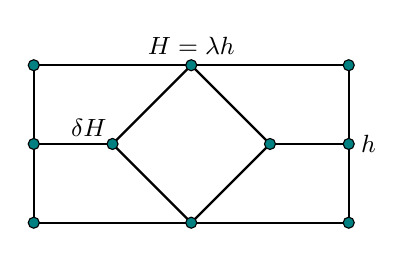
\begin{tikzpicture}
%\draw[fill=gray!23,gray!23](0,0) rectangle (5,5);
%\draw[step=0.5cm,gray,very thin] (0,0) grid (6,4); %background grid
\draw[thick] (1,1) -- (5,1) -- (5,3) -- (1,3) -- cycle;  
\draw[thick] (3,1) -- (4,2) -- (3,3) -- (2,2) -- cycle;  
\draw[thick] (1,2) -- (2,2);  
\draw[thick] (4,2) -- (5,2);  
\node[] at (5.25,2) {\small $h$};
\node[] at (3,3.25) {\small $H=\lambda h$};
\node[] at (1.7,2.2) {\small $\delta H$};
\draw[black,fill=teal] (1,1) circle (2pt);
\draw[black,fill=teal] (3,1) circle (2pt);
\draw[black,fill=teal] (5,1) circle (2pt);
\draw[black,fill=teal] (1,2) circle (2pt);
\draw[black,fill=teal] (2,2) circle (2pt);
\draw[black,fill=teal] (4,2) circle (2pt);
\draw[black,fill=teal] (5,2) circle (2pt);
\draw[black,fill=teal] (1,3) circle (2pt);
\draw[black,fill=teal] (3,3) circle (2pt);
\draw[black,fill=teal] (5,3) circle (2pt);
\end{tikzpicture}
\end{center}

The total area is 
\[
A= \lambda h \cdot h = \lambda h^2
\]
The area of the trapezes is
\[
A_{TR} = (\frac{H}{2} + \delta H)\frac12 \cdot \frac{h}{2}=\frac{\lambda h^2}{4} \left(\frac12 + \delta \right)
\]
while the area of the middle diamond is
\[
A_D = 4 \cdot \frac12 \frac{h}{2} \left(\frac{H}{2}-\delta H \right) 
= \lambda h^2 \left(\frac12 - \delta \right)
\]
We can compute $\delta$ by requiring that the trapezes and the diamond all 
have the same area, i.e.
\[
\frac{\lambda h^2}{4} (\frac12 + \delta)
=
\lambda h^2 (\frac12 - \delta)
\qquad
\Rightarrow \quad \delta = 0.3
\]
We find that the value of $\delta$ is independent of $\lambda$.

We see in the literature \cite{sten84,brfo,chba93}  that the 
macro-element is often depicted with the diamond being a square.
In this case we must have along the horizontal middle line
\[
\lambda h = 0.3 \lambda h + \frac{h}{2}+ \frac{h}{2} + 0.3 \lambda h
\qquad
\Rightarrow \quad 
\lambda=5/2
\]
The 5:2 aspect ratio macro-element guarantees equal areas and a square middle element.

But does the aspect ratio matter in practice? no. D\&H tests indicate
small differences in velocity and pressure errors between 1:1 and 5:2 aspect ratios.

\item LT: let us isolate one fourth of this macro-element:

\begin{center}
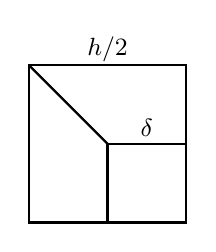
\begin{tikzpicture}
\draw[thick] (1,1) -- (3,1) -- (3,3) -- (1,3) -- cycle;  
\draw[thick] (1,3) -- (2,2);  
\draw[thick] (2,1) -- (2,2) --(3,2);  
\node[] at (2.5,2.2) {\small $\delta$};
\node[] at (2,3.2) {\small $h/2$};
\end{tikzpicture}
\end{center}

The area of the trapezes is 
\[
A_{TR}=\frac12 (\frac{h}{2}+\delta) (\frac{h}{2}-\delta) = \frac{h^2}{8}- \frac{\delta^2}{2}
\]
while the area of the square element is $A_{SQ}=\delta^2$.
When set to be equal, we arrive at
\[
\delta = \frac{h}{\sqrt{12}} \simeq 0.288 h
\]
Again, looking at velocity and pressure errors we find that 
these are mildly dependent on $\delta$. 

\item QZ1. I need to type my notes. We can build a 
macro-element with equal area elements if $\epsilon=h/\sqrt{6}$

\item QZ2: not possible to build macro-element of equal area elements. 
I set $\epsilon=h/5$

\item QZ3. I need to type my notes. We can build a 
macro-element with equal area elements if $\epsilon=h/6$

\item T1: not possible to build macro-element of equal area elements. 
I set $\epsilon=h/2/\sqrt{5}$

\item T2. I need to type my notes. We can build a 
macro-element with equal area elements if $\epsilon=h/2/\sqrt{5}$
 
\end{itemize}


\newpage



\begin{center}
\includegraphics[width=4.3cm]{../images/4x4/topos.0000.png}
\includegraphics[width=4.3cm]{../images/4x4/topos.0008.png}
\includegraphics[width=4.3cm]{../images/4x4/topos.0009.png}
\includegraphics[width=4.3cm]{../images/4x4/topos.0010.png}\\
\includegraphics[width=4.3cm]{../images/4x4/topos.0001.png}
\includegraphics[width=4.3cm]{../images/4x4/topos.0002.png}
\includegraphics[width=4.3cm]{../images/4x4/topos.0003.png}
\includegraphics[width=4.3cm]{../images/4x4/topos.0004.png}\\
\includegraphics[width=4.3cm]{../images/4x4/topos.0005.png}
\includegraphics[width=4.3cm]{../images/4x4/topos.0006.png}
\includegraphics[width=4.3cm]{../images/4x4/topos.0007.png}\\
4x4 macro-element meshes for R, Rp, Rrp, FR, S, LT, QZ1, QZ2, QZ3, T1, T2.
\end{center}



\end{document}
